\documentclass[11pt]{article}
\usepackage[margin=1in]{geometry}
\usepackage{fontspec}
\setmainfont{Times New Roman}
\setsansfont{Arial}
\usepackage{amsmath,amssymb,graphicx,mathtools}
\usepackage[unicode,hidelinks]{hyperref}
\usepackage{microtype}
\usepackage{float,caption}
\captionsetup{font=small,labelfont=bf}
\setlength{\parindent}{0pt}
\setlength{\emergencystretch}{3em}
\title{Modelling Antibody Therapy Dynamics with Applications to Glofitamab: A Summary of Experiments :)}
\author{}
\date{June 8, 2026}
\begin{document}
\maketitle
\section*{Abstract}

Bispecific antibody therapies enable a powerful targeted immune activation against tumor cells, but are frequently limited by severe toxicities arising from poorly understood links between drug exposure, immune activation, and downstream cytokine dynamics. We replicated and built on models from many papers, using a mechanistic and computational framework to study bispecific antibody behavior, with a focus on Glofitamab, a CD20CD3 T-cell engaging therapy used in lymphoma treatment. 
\par\medskip

We first conduct a comprehensive literature review spanning three modeling paradigms: full kinetic mass-action ordinary differential equation (ODE) models, quasi-equilibrium (QE) differential algebraic equation (DAE) models, and pharmacokinetic/pharmacodynamic (PK/PD) frameworks. Building on these foundations, we replicate key models using Python and MATLAB/Simulink and construct extended models that capture multivalent binding, ternary complex formation, and downstream immune side effects. 
\par\medskip

Our simulations demonstrate that avidity-driven interactions enable sustained target engagement, while engineered affinity asymmetry limits systemic T-cell activation. We further demonstrate that cytokine release syndrome (CRS) severity is driven primarily by peak ternary complex formation rather than total drug exposure, highlighting the importance of early binding dynamics. In addition, we propose an IL-6 centered weight loss mechanism in which treatment associated inflammatory signaling contributes to both fat loss and lean mass loss through anorexia, adipose lipolysis/browning, and skeletal muscle catabolism, distinguishing short term cytokine driven appetite suppression from longer term cachexia like tissue wasting, providing a basis for future modeling and experimental validation. Overall, this work establishes a reproducible and mechanistic framework for analyzing bispecific antibody therapies and offers quantitative insights for optimizing Glofitamab dosing strategies to balance efficacy and toxicity.
\par\medskip

\section{Background}

\subsection{Bispecific Antibodies and Glofitamab Mechanism}

Bispecific antibodies, such as Glofitamab, represent a rapidly advancing class of targeted therapeutics that simultaneously bind two distinct targets and enable interaction between immune effector cells and tumor cells. Glofitamab is a 2:1 bispecific monoclonal antibody commonly used to treat types of B-cell lymphomas, a class of cancers originating in B lymphocytes that can affect lymph nodes, blood, bone marrow, the central nervous system, bones, and other tissues. It functions by simultaneously binding CD20 on B cells and CD3 on T-cells, bringing them into close proximity and creating a ternary complex. This interaction creates a physical link between tumor cells and T-cells, leading to targeted T-cell-mediated cytotoxicity. However, once formed, this structure also forces abnormal T-cell activation that bypasses normal mechanisms of immune regulation, triggering a rapid release of inflammatory cytokines and putting the patient at risk of CRS.
\par\medskip

\subsection{Clinical Limitation: Cytokine Release Syndrome}

As a result, CRS represents a major clinical limitation of T-cell-engaging bispecific antibodies, motivating the need for predictive and mechanistic modeling approaches. CRS is a systemic inflammatory response which commonly follows immune-based therapies such as bispecific antibodies. This response arises from rapid and unregulated immune activation, leading to the release of pro-inflammatory cytokines. Interleuking-6 (IL-6) often serves as a key clinical biomarker of CRS severity. Previous studies have shown that cytokine release in CD3 T-cell engager therapies is directly tied to immune activation mechanisms rather than just drug concentration [1]. Similarly, CAR T-cell modeling work shows that cytokine production depends on activated immune cell populations and their interactions [2].
\par\medskip

After the ternary complex forms, cytokine release happens quickly. IL-6 levels typically rise sharply and then decrease as the cytokine is cleared from the bloodstream. The peak level of IL-6 is especially important, since it is closely linked to the severity of CRS. Clinical evidence supports this, noting that “real-time interleukin-6 (IL-6) kinetics predict cytokine release syndrome (CRS) [3]”. Importantly, CRS severity is more strongly related to the peak level of immune activation (i.e., ternary complex concentration) rather than the total amount of drug given.
\par\medskip

\begin{figure}[H]
\centering
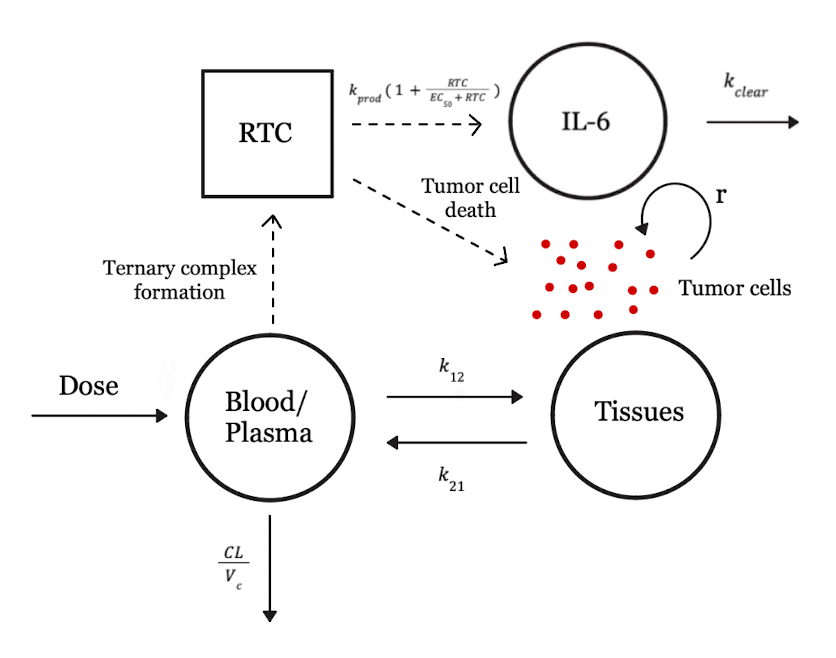
\includegraphics[width=\linewidth,height=.65\textheight,keepaspectratio]{figures/original_00.png}
\caption{Simplified schematic of mechanistic PK/PD model linking drug pharmacokinetics, ternary complex formation, cytokine release, and tumor dynamics based on the simplified IL-6 model and separated ODE system}
\label{fig:original-00}
\end{figure}

Mechanistically, CRS is initiated as therapeutic agents promote the formation of complexes bridging T-cells and target cells, resulting in T-cell activation, cytokine secretion, and cytotoxic activity. While important for anti-tumor efficacy, these processes can result in significant toxicity when dysregulated. As such, understanding and predicting cytokine dynamics is critical for optimizing therapeutic dosing strategies that balance efficacy and side effect risk mitigation.
\par\medskip

\section{Literature Review}

\subsection{Modeling Frameworks for Antibody Therapy Dynamics}

To address these challenges and better predict toxicity and therapeutic efficacy, a range of modeling frameworks have been developed to describe antibody therapy dynamics. There are three primary classes of models, each spanning different levels of mechanistic detail and computational complexity. The first classification consists of full kinetic mass-action ODE models, which explicitly represent cell-surface binding interactions. These models explicitly represent receptor-ligand association and dissociation, internalization, recycling, and turnover using coupled ODEs. For bispecific antibodies, this typically includes formation of binary complexes and ternary complexes. Because all kinetic steps are modeled directly, mass-action systems can capture transient behaviors such as time dependent target engagement, competition, and saturation.
\par\medskip

The second class comprises QE multivalent binding models formulated as DAE systems, which approximate fast binding dynamics using equilibrium relationships. When binding is fast relative to distribution, internalization, and turnover, we can approximate binding as relatively instantaneous. This replaces the fastest ODE dynamics with algebraic equilibrium relationships, producing DAEs. These formulations can dramatically reduce stiffness and parameter sensitivity while still retaining key nonlinearities.
\par\medskip

The final class consists of mechanistic PK/PD models for bispecifics. At the whole body scale, and within the context of this project, compartmental PK/PD frameworks describe antibody absorption, distribution between plasma and tissues, lymphatic transport, and elimination, while linking these processes to pharmacodynamic effects such as tumor killing and cytokine release. These models are well suited for dose and regimen exploration and translation across species and patient populations. However, they require careful assumptions about tissue structure, permeability, and target expression heterogeneity. Together, these three approaches underscore the need for integrated frameworks capable of capturing multivalent binding, immune activation, and clinically relevant outcomes, particularly those associated with CRS.
\par\medskip

\subsection{Mass-Action ODE Models for Bispecific Binding}

Mass-action ODE models provide a detailed mechanistic framework for describing antibody-receptor interactions at the cellular level. Ray et al. [4] developed a mechanistic computational framework to compare monospecific antibodies with bispecific antibodies that can bind two distinct receptor targets simultaneously, focusing on a representative bispecific design (BS1) targeting IL-6 and IL-8 receptor systems. Using this setup, they argue that bispecific binding can produce more efficient functional engagement than monospecific approaches because a single molecule can coordinate interactions across two receptor types rather than acting independently on one target at a time.
\par\medskip

A central contribution of the paper is a kinetic mass-action ODE model of cell-surface receptor–antibody binding, constructed to explicitly track the full set of interacting species over time.
\par\medskip

\begin{figure}[H]
\centering
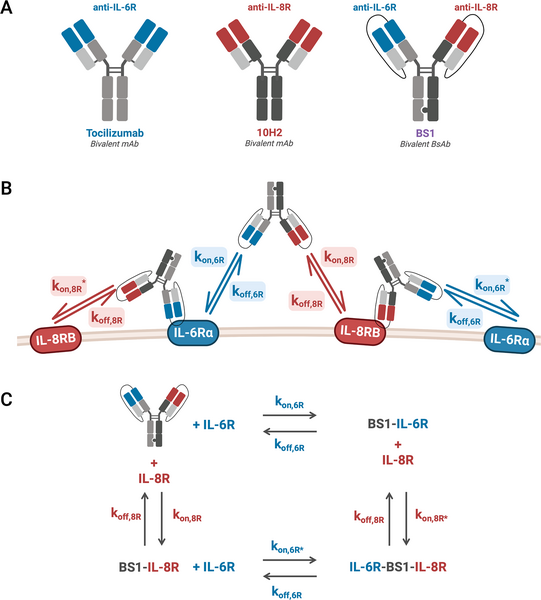
\includegraphics[width=\linewidth,height=.65\textheight,keepaspectratio]{figures/original_01.png}
\caption{Schematic representations of mono- and bispecific antibody binding interactions and reaction kinetics. (A) Structural representation of monoclonal antibodies targeting IL-6R or IL-8R and a bispecific antibody. (B) Reversible binding interactions between antibodies and receptors governed by rate constants. (C) Simplified binding pathways demonstrating interconversion between free receptors, binary complexes, and ternary complexes [4].}
\label{fig:original-01}
\end{figure}

The binding model is given by Equation~\ref{eq:binary-binding} and Equation~\ref{eq:ternary-binding}:
\begin{equation}
\begin{aligned}
\frac{d[R_1\cdot Ab]}{dt}
&= k_{\mathrm{on},R_1}[R_1][Ab]
 + k_{\mathrm{off},R_2^{*}}[R_1\cdot Ab\cdot R_2] \\
&\quad - k_{\mathrm{on},R_2^{*}}[R_2][R_1\cdot Ab]
 - k_{\mathrm{off},R_1}[R_1\cdot Ab].
\end{aligned}
\label{eq:binary-binding}
\end{equation}
\begin{equation}
\begin{aligned}
\frac{d[R_1\cdot Ab\cdot R_2]}{dt}
&= k_{\mathrm{on},R_1^{*}}[R_1][R_2\cdot Ab]
 + k_{\mathrm{on},R_2^{*}}[R_2][R_1\cdot Ab] \\
&\quad - k_{\mathrm{off},R_1^{*}}[R_1\cdot Ab\cdot R_2]
 - k_{\mathrm{off},R_2^{*}}[R_1\cdot Ab\cdot R_2].
\end{aligned}
\label{eq:ternary-binding}
\end{equation}

\emph{Equation~\ref{eq:binary-binding} and Equation~\ref{eq:ternary-binding} describe sequential antibody binding, where initial receptor engagement forms a binary complex followed by cross-linking to a second receptor to form a ternary complex [4].}
\par\medskip

\subsection{Multivalent Binding and Avidity Effects}

A key extension of mass-action frameworks is the incorporation of multivalent binding and avidity effects. Rhoden et al. [5] combine a mechanistic mass action ODE model of multivalent/bispecific binding with quantitative cell based receptor occupancy experiments to explain how antigen density and the expression ratio of two targets on the same cell can make “effective binding” differ dramatically from 1:1 monovalent affinity (sometimes by orders of magnitude).
\par\medskip

The avidity model is given by Equation~\ref{eq:avidity-antibody} through Equation~\ref{eq:avidity-double}.
\begin{equation}
\begin{aligned}
\frac{d[Ab]}{dt} &= -k_{\mathrm{on}}^{Ag1}[Ag1][Ab]-k_{\mathrm{on}}^{Ag2}[Ag2][Ab]\\ &\quad+k_{\mathrm{off}}^{Ag1}[B_{Ag1}]+k_{\mathrm{off}}^{Ag2}[B_{Ag2}].
\end{aligned}
\label{eq:avidity-antibody}
\end{equation}
\begin{equation}
\begin{aligned}
\frac{d[Ag1]}{dt} &= -k_{\mathrm{on}}^{Ag1}[Ag1][Ab]+k_{\mathrm{off}}^{Ag1}[B_{Ag1}]\\ &\quad-k_{\mathrm{on}}^{Ag1}[Ag1_{\mathrm{eff}}]\frac{[Ag1]}{[Ag1_0]}[B_{Ag2}]+k_{\mathrm{off}}^{Ag1}[B_{\mathrm{dbl}}].
\end{aligned}
\label{eq:avidity-ag1}
\end{equation}
\begin{equation}
\begin{aligned}
\frac{d[Ag2]}{dt} &= -k_{\mathrm{on}}^{Ag2}[Ag2][Ab]+k_{\mathrm{off}}^{Ag2}[B_{Ag2}]\\ &\quad-k_{\mathrm{on}}^{Ag2}[Ag2_{\mathrm{eff}}]\frac{[Ag2]}{[Ag2_0]}[B_{Ag1}]+k_{\mathrm{off}}^{Ag2}[B_{\mathrm{dbl}}].
\end{aligned}
\label{eq:avidity-ag2}
\end{equation}
\begin{equation}
\begin{aligned}
\frac{d[B_{Ag1}]}{dt} &= k_{\mathrm{on}}^{Ag1}[Ag1][Ab]-k_{\mathrm{off}}^{Ag1}[B_{Ag1}]\\ &\quad-k_{\mathrm{on}}^{Ag2}[Ag2_{\mathrm{eff}}]\frac{[Ag2]}{[Ag2_0]}[B_{Ag1}]+k_{\mathrm{off}}^{Ag2}[B_{\mathrm{dbl}}].
\end{aligned}
\label{eq:avidity-bag1}
\end{equation}
\begin{equation}
\begin{aligned}
\frac{d[B_{Ag2}]}{dt} &= k_{\mathrm{on}}^{Ag2}[Ag2][Ab]-k_{\mathrm{off}}^{Ag2}[B_{Ag2}]\\ &\quad-k_{\mathrm{on}}^{Ag1}[Ag1_{\mathrm{eff}}]\frac{[Ag1]}{[Ag1_0]}[B_{Ag2}]+k_{\mathrm{off}}^{Ag1}[B_{\mathrm{dbl}}].
\end{aligned}
\label{eq:avidity-bag2}
\end{equation}
\begin{equation}
\begin{aligned}
\frac{d[B_{\mathrm{dbl}}]}{dt} &= k_{\mathrm{on}}^{Ag1}[B_{Ag2}][Ag1_{\mathrm{eff}}]\frac{[Ag1]}{[Ag1_0]}\\ &\quad+k_{\mathrm{on}}^{Ag2}[B_{Ag1}][Ag2_{\mathrm{eff}}]\frac{[Ag2]}{[Ag2_0]}\\ &\quad-\left(k_{\mathrm{off}}^{Ag1}+k_{\mathrm{off}}^{Ag2}\right)[B_{\mathrm{dbl}}].
\end{aligned}
\label{eq:avidity-double}
\end{equation}

\begin{equation}
\begin{aligned}
Ab + Ag1
&\mathrel{\mathop{\rightleftarrows}\limits^{k_{\mathrm{on}}^{Ag1}}_{k_{\mathrm{off}}^{Ag1}}}
B_{Ag1}, \
\end{aligned}
\label{eq:reaction-1}
\end{equation}
\begin{equation}
\begin{aligned}
Ab + Ag2
&\mathrel{\mathop{\rightleftarrows}\limits^{k_{\mathrm{on}}^{Ag2}}_{k_{\mathrm{off}}^{Ag2}}}
B_{Ag2}, \
\end{aligned}
\label{eq:reaction-2}
\end{equation}
\begin{equation}
\begin{aligned}
B_{Ag1} + Ag2^{\mathrm{surf}}
&\mathrel{\mathop{\rightleftarrows}\limits^{k_{\mathrm{on}}^{Ag2}}_{k_{\mathrm{off}}^{Ag2}}}
B_{\mathrm{dbl}}, \
\end{aligned}
\label{eq:reaction-3}
\end{equation}
\begin{equation}
\begin{aligned}
B_{Ag2} + Ag1^{\mathrm{surf}}
&\mathrel{\mathop{\rightleftarrows}\limits^{k_{\mathrm{on}}^{Ag1}}_{k_{\mathrm{off}}^{Ag1}}}
B_{\mathrm{dbl}}.
\end{aligned}
\label{eq:reaction-4}
\end{equation}

Equation~\ref{eq:avidity-antibody} through Equation~\ref{eq:avidity-double} describe antibody-antigen dynamics; Equation~\ref{eq:reaction-1} through Equation~\ref{eq:reaction-4} show the corresponding reversible binding reactions. \emph{[5]}
\par\medskip

\subsection{Quasi-Equilibrium Multivalent Binding Models}

Ng and Bauer [6] utilize a QE binding model which is implemented using DAEs instead of kinetic ODEs. The authors assume fast binding in kinetics equilibrates instantly in relation to the PK processes. The processes are then separated into two timescales, slow (in cases such as drug distribution, elimination, and receptor turnover) and fast (such as drug-receptor binding).
\par\medskip

The different ways biologics are able to bind constitute their pharmacokinetics  and pharmacodynamics. Biologics refer to complex and different groups of molecules that have diverse binding kinetics to receptors such as IgG, bispecific antibodies, and antibodies, each with different capabilities as to how many different receptors they can bind to at a time. Previous models have been created that show how drug receptor binding occurs and models the drug binding kinetics’ effects on PK and PD behaviors. These models were created with ODEs with rates of dissociation between drugs and receptors. The rates of dissociation however are hard to estimate because binding can be quicker than elimination and distribution. Additionally there are previously constructed QE  models, but they have only taken into account drug-receptor interactions that can only bind one-to-one. Other such models have been created such as quasi-steady-state (QSS), yet each need intense mathematical derivations and cannot be generalized and applied in different instances without additional changes to the preexisting models. This study aims to construct a DAE based QE multivalent drug-receptor binding model to apply to different and complex drug receptor interactions of biologics with the goals of it being applicable across bispecific antibodies, IgG molecules, and anti-VEGF IgG monoclonal antibodies, in which each type can bind to different amounts of receptors.
\par\medskip

\subsection{Structural Design and Mechanism of Action of Bispecific Antibodies}

Madsen et al. [7] review the key structural and engineering principles that govern the design of bispecific antibodies, emphasizing that their therapeutic advantages arise directly from their dual-binding capability. Bispecific antibodies enable “simultaneous targeting of antigens and synergetic binding effects beyond what can be obtained even with combinations of conventional monospecific antibodies [7]”. However, this benefit comes with increased structural complexity compared to monospecific IgGs. The authors note that bispecific antibody development is frequently challenged by “decreased biophysical stability from fusion of exogenous antigen-binding domains” and “antibody chain mispairing [leads] to formation of antibody-related impurities that are very difficult to remove [7]”. As a result, bispecific antibody construction requires careful molecular engineering to ensure correct chain pairing, structural integrity, and favorable drug-like properties. This highlights that therapeutic performance is inseparable from structural design and manufacturability.
\par\medskip

\begin{figure}[H]
\centering
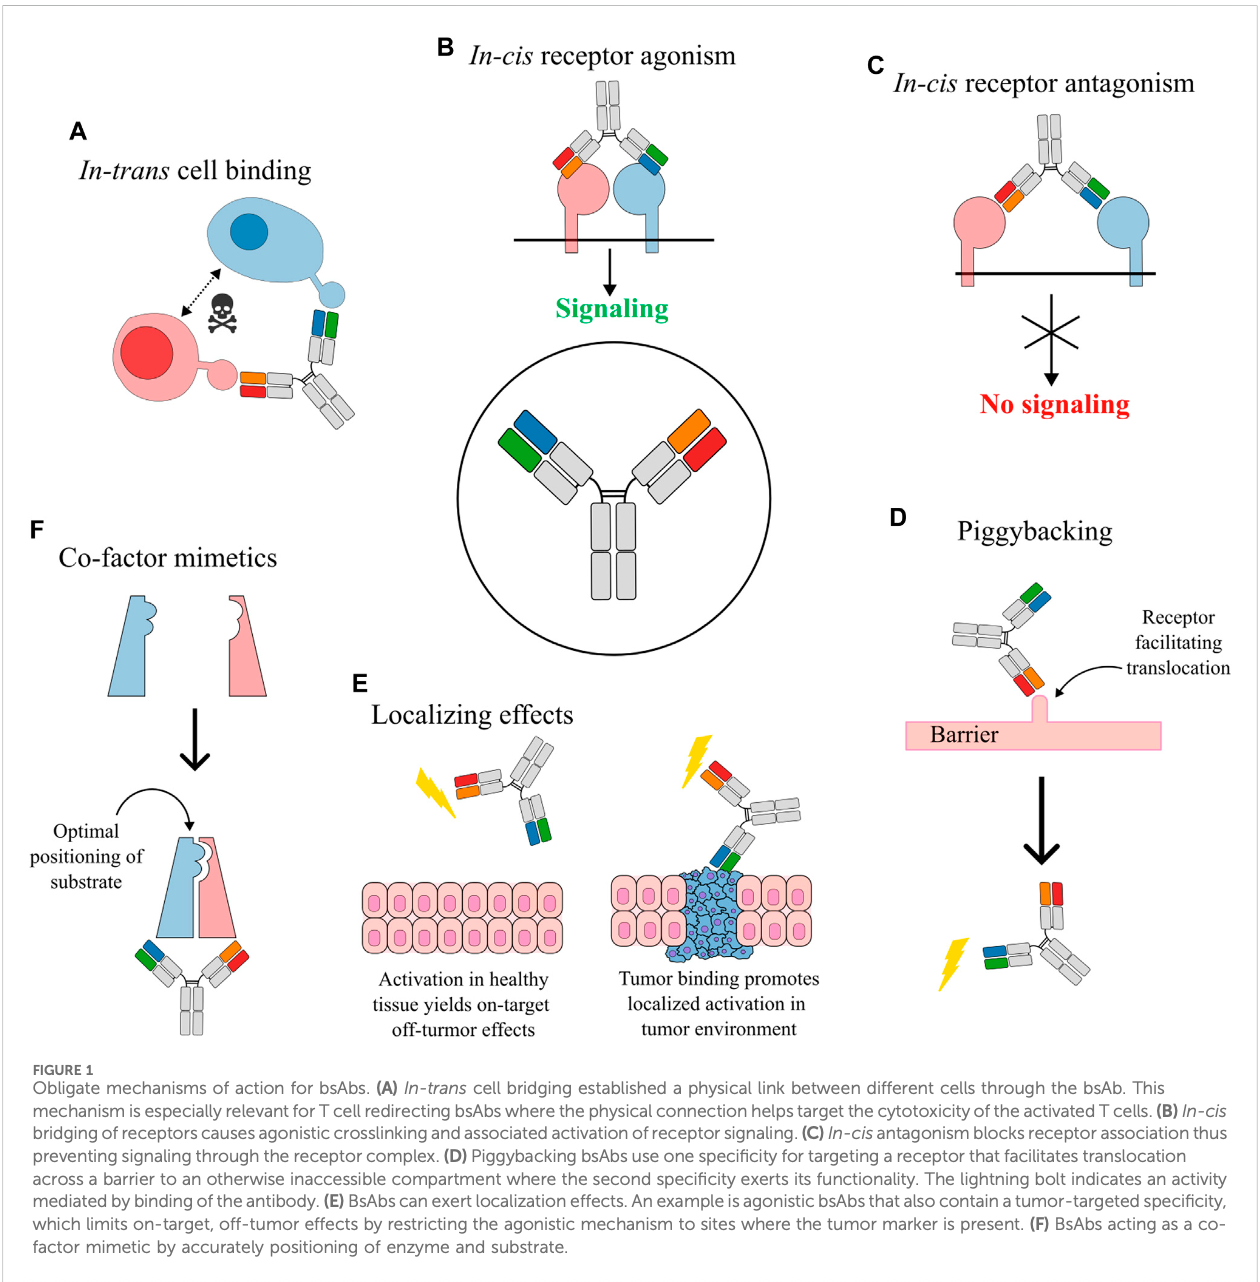
\includegraphics[width=\linewidth,height=.65\textheight,keepaspectratio]{figures/original_05.png}
\caption{Mechanisms of bispecific antibody action, including cell bridging, receptor modulation, targeted localization, transport across barriers, and cofactor mimicry [7].}
\label{fig:original-05}
\end{figure}

\begin{figure}[H]
\centering
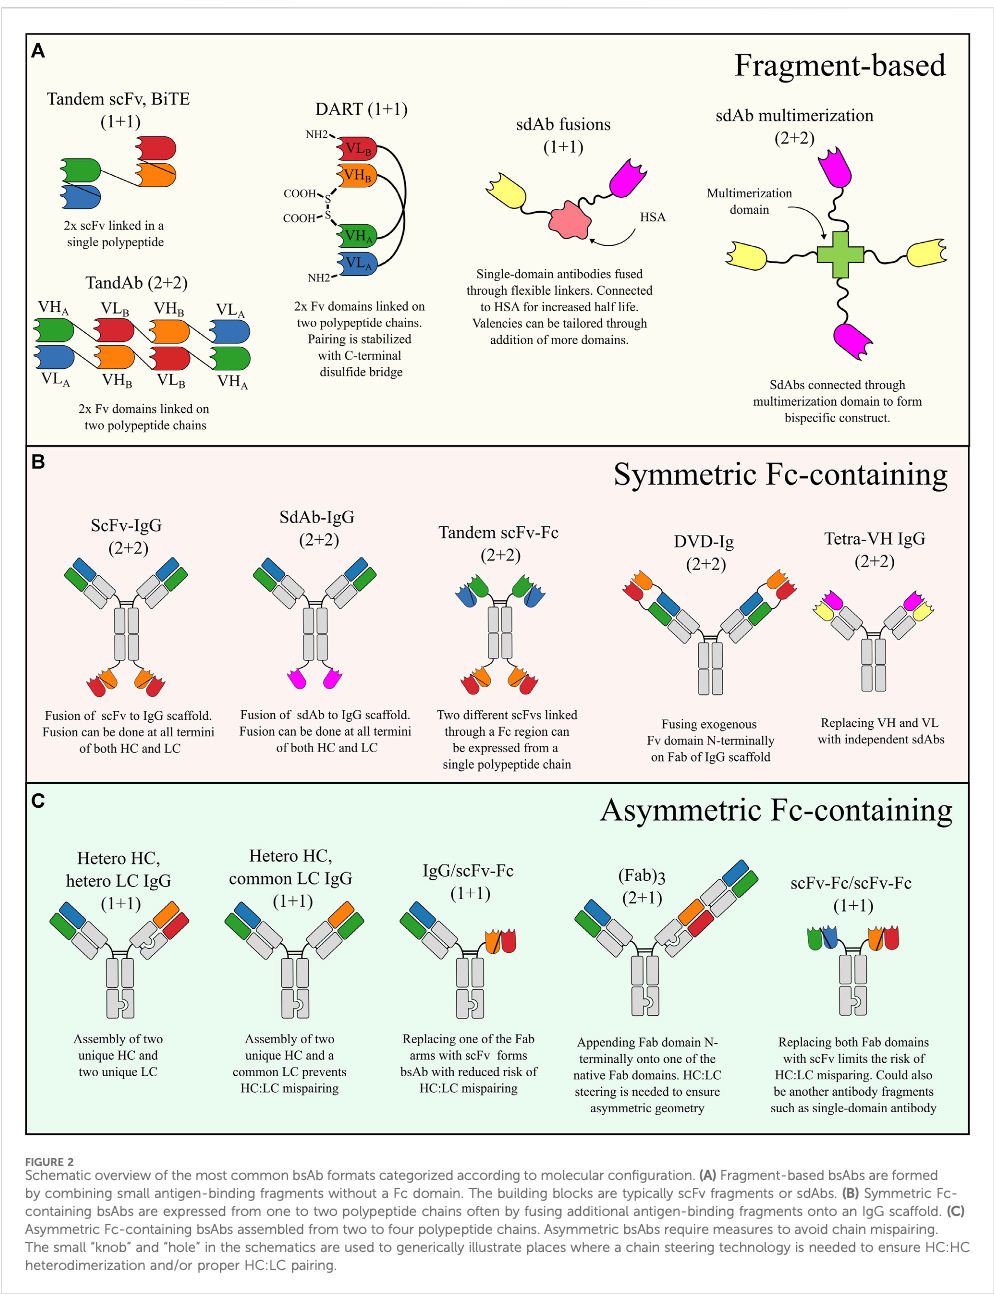
\includegraphics[width=\linewidth,height=.65\textheight,keepaspectratio]{figures/original_06.png}
\caption{Structural classes of bispecific antibodies, including fragment-based, symmetric Fc-containing, and asymmetric Fc-containing formats [7].}
\label{fig:original-06}
\end{figure}

A central part of the paper is the emphasis on mechanism of action and spatial configuration. The authors explain that for many bispecific antibodies, efficacy depends on a precise “spatiotemporal connection between the two binding events” meaning that “the two binding specificities must be engaged in a specific physical arrangement…and/or with a specific timing [7]”. \emph{Figure~\ref{fig:original-05}} illustrates key obligate mechanisms, including in-trans cell bridging and in-cis receptor agonism or antagonism, demonstrating how geometry and target positioning directly influence biological outcomes. Additionally, \emph{Figure~\ref{fig:original-06}}\textbf{ }categorizes major molecular formats like symmetric Fc-containing and asymmetric Fc-containing constructors which affect stability, valency, and chain-pairing risk.
\par\medskip

\subsection{Cytokine Dynamics and CRS Mechanisms}

Although IL-6 is commonly used as the primary biomarker for CRS, it does not always fully capture the severity of the immune response. More recent studies suggest that other cytokines, particularly IL-10 and interferon-gamma (IFN-γ), may be better indicators depending on the therapy being used. For example, one paper states that “IL-6 trended with CRS for mosunetuzumab tebentafusp and tarlatamab, but IL-10 and IFN-γ better trended with CRS for glofitamab and elranatamab [8]”. Mechanistically, Glofitamab induces a rapid pharmacodynamic response that is characterized by early T-cell activation and cytokine release, with IFN-γ and IL-10 appearing to be the cytokines most closely aligned with CRS onset. In a phase 1 study, Glofitamab caused dose-dependent induction of inflammatory cytokines right after the first infusion with IFN-γ peaking at the end of infusion, whereas IL-6 peaks later at approximately six hours after infusion. IL-10 was also rapidly induced alongside these early cytokines, indicating that it participates in the initial immune activation phase rather than only a delayed regulatory response. This supports the conclusion that IFN-γ and IL-10 are a better fit for modeling glofitamab-driven CRS, since these cytokines more directly reflect early T-cell activation phases rather than the later downstream signal of the macrophage-amplified inflammatory cascade [8]. This shows that CRS should not be treated as a single-cytokine problem, but rather as a system involving multiple interacting cytokines. \newline{}\newline{}From a modeling perspective, IL-10 and IFN-γ can be incorporated using a similar structure to IL-6, with production and clearance terms coupled to immune cell populations. In CAR T-cell models, cytokine dynamics are described using ordinary differential equations (ODEs) that account for both cytokine production and decay, as well as their relationship to immune activation [2]. In these models, activated T cells and monocytes are the main drivers of IL-10 and IFN-γ production, which means their levels depend directly on immune activation. The models also introduce the idea of a combined cytokine burden that correlates CRS severity, rather than relying on a single cytokine measurement. \newline{}\newline{}These CAR-T based models are useful starting points for bispecific antibody modeling because their structure can be adapted. For example, CAR-T cell counts can be replaced with activated T-cell populations, and monocyte dynamics can be modified to represent macrophage or general immune activation states. Additionally, these models provide reasonable estimates for cytokine production and decay rates, along with reference concentration ranges for mild versus severe CRS. While the numerical values may differ due to differences in exposure time between CAR-T and bispecific therapies, general properties such as decay rates and equation structure can still be applied.
\par\medskip

Further understanding of IL-10 and IFN-γ comes from studies of cytokine storms, which focus on how different cytokines interact over time. These studies show that IL-10 and IFN-γ operate on different timescales and have different roles in the immune response. IFN-γ acts as an early pro-inflammatory driver, increasing rapidly after immune activation and helping amplify the overall response. In contrast, IL-10 appears later and functions as part of a regulatory system that reduces inflammation. As described in one study, IFN-γ is an early driver while IL-10 is part of a later regulatory cluster [9]. IL-10 also has inhibitory effects on other cytokines, meaning it helps dampen the overall immune response once it has been activated.
\par\medskip

This regulatory role of IL-10 is also supported by reduced inflammatory response models. These models describe anti-inflammatory mediators such as cortisol and IL-10 that suppress pro-inflammatory signaling. In these frameworks, IL-10 is produced in response to immune activation and tissue damage, and then decays over time through first-order kinetics. Its main effect is to reduce the activity of pro-inflammatory cytokines, often through nonlinear inhibition such as Hill-type functions. This type of structure can be directly incorporated into CRS models as a feedback mechanism.
\par\medskip

In addition to its role in cytokine signaling, IL-10 also affects immune cell behavior. For example, it has been shown to act as a down regulator of T-cell expansion and macrophage phenotypes, which further supports its role in limiting excessive immune activation [10]. Overall, this suggests that IL-10 acts as a stabilizing component in the system, while IFN-γ acts as an amplifying component.
\par\medskip

Based on these findings, a more complete CRS model should include both positive and negative mechanisms. IFN-γ contributes to early immune activation and amplification of cytokine release, while IL-10 provides delayed negative feedback that helps control and resolve inflammation. Incorporating both cytokines allows the model to better reproduce the characteristic rise-and-fall behavior of cytokine levels during CRS. However, these additions still require calibration using clinical data, particularly for Glofitamab, in order to accurately match observed cytokine levels and CRS grading.
\par\medskip

\subsection{Weight Loss Mechanisms}

Weight loss in this system arises from two overlapping sources: the underlying cancer/cachexia state and treatment associated inflammatory signaling. For modeling purposes, this distinction matters because acute cytokine elevations during CRS are most likely to capture short term anorexia and sickness behavior, whereas larger, progressive body weight decline is more consistent with chronic cachexia, which involves ongoing loss of both fat and lean tissue rather than reduced intake alone [11, 12, 13]. This has also been clinically supported by a CAR T-cell lymphoma study, which found that recent pre-treatment weight loss was associated with higher inflammatory markers, including IL-6, and with poorer outcomes, suggesting that weight loss should be treated as a meaningful inflammatory disease state rather than a trivial side effect [14].
\par\medskip

A major mechanism is IL-6 driven skeletal muscle wasting. Chronic IL-6 has been identified as a critical inflammatory mediator in cancer cachexia and is strongly linked to loss of muscle mass [15]. More specifically, it has been shown that IL-6 overexpression can accelerate body weight loss and muscle wasting, while IL-6 receptor blockade can improve mitochondrial content and attenuated progression of cachexia [16]. Mechanistically, this muscle loss pathway involves proteolysis, autophagy, and mitochondrial dysfunction: early in cachexia, PGC-1α, Mfn1, and Mfn2 are suppressed, and with progressive wasting, FIS1 increases, supporting a shift toward impaired mitochondrial maintenance and a more catabolic muscle state [16]. Thus, IL-6 is not simply associated with weakness, it plausibly contributes directly to the lean mass component of weight loss through muscle proteolysis and mitochondrial remodeling [15, 16].
\par\medskip

A second major mechanism is IL-6 driven adipose depletion. In a study with cachectic patients, serum IL-6 was positively associated with serum free fatty acids, supporting a link between IL-6 and adipose lipolysis [12]. This same study found that white adipose tissue lipolysis is elevated in early cachexia, whereas white adipose browning is more evident in late cachexia, therefore suggesting a progression from early fat mobilization to later thermogenic energy wasting [12]. Importantly, blocking IL-6 signaling with anti-IL-6R inhibited lipolysis and browning, and partially preserved fat mass in cachectic mice, indicating that IL-6 is a strong candidate driver of the fat loss component of weight loss [12]. This has been corroborated in the literature, describing chronic IL-6 as promoting lipolysis, browning, insulin resistance, and negative energy balance in cachexia [11].
\par\medskip

In addition to these tissue effects, the reviewed literature supports a central hypothalamic mechanism that can further amplify weight loss. Cachexia is described as a state produced by a “synergistic combination” of decreased appetite and increased metabolism of fat and lean body mass [13]. The hypothalamus contains anorexigenic POMC/CART neurons and orexigenic AgRP/NPY neurons, and cytokine signaling shifts this system towards reduced feeding and greater catabolic output [13, 17]. More broadly, hypothalamic inflammation is described as a key driver of anorexia, lethargy, altered energy balance, and downstream catabolism, with the HPA axis and related neuroendocrine pathways promoting adipose lipolysis and skeletal muscle proteolysis [17]. An IL-6 specific version of this pathway is further supported, as IL-6 can suppress appetite by inhibiting NPY/AgRP neurons and stimulating POMC neurons while also increasing energy expenditure [11]. Therefore, any observed weight loss can be understood as the result of both reduced intake and active inflammatory tissue wasting, not appetite loss or weakness alone [13, 17].
\par\medskip

Taken together, the literature supports representing body weight as the sum of at least two biological compartments, namely fat mass and lean mass, with an additional central regulatory effect for hypothalamic appetite and energy balance signaling. In this framework, chronic IL-6 contributes to fat loss through lipolysis and browning, to muscle loss through proteolysis, autophagy, and mitochondrial dysfunction, and to further weight decline through centrally mediated anorexia and increased energy expenditure [12, 13, 16, 17]. Accordingly, modeling CRS associated IL-6 is most appropriate for capturing short term appetite suppression and sickness behavior, whereas long term progressive weight loss is more plausibly explained by a sustained IL-6 centered cachexia process. The literature reviewed supports an inflammatory cachexia mechanism as the main explanation for weight loss. Based on these findings, a possible model is given below.
\par\medskip


\begin{equation}
\begin{aligned}
W(t) &= F(t)+L(t).
\end{aligned}
\label{eq:body-weight}
\end{equation}

\emph{Equation~\ref{eq:body-weight} expresses total body weight as the sum of fat mass and lean mass.}
\par\medskip


\begin{equation}
\begin{aligned}
\frac{dF}{dt} &= k_{F,\mathrm{in}}I(H)-\left(k_{F,0}+k_{F,\mathrm{IL6}}\frac{\mathrm{IL6}}{K_F+\mathrm{IL6}}+k_{FB}B\right)F.
\end{aligned}
\label{eq:fat-mass}
\end{equation}
\begin{equation}
\begin{aligned}
\frac{dL}{dt} &= k_{L,\mathrm{in}}I(H)-\left(k_{L,0}+k_{L,\mathrm{IL6}}\frac{\mathrm{IL6}}{K_L+\mathrm{IL6}}+k_{LM}M\right)L.
\end{aligned}
\label{eq:lean-mass}
\end{equation}
\begin{equation}
\begin{aligned}
\frac{dB}{dt} &= a_B\frac{\mathrm{IL6}}{K_B+\mathrm{IL6}}-d_BB.
\end{aligned}
\label{eq:browning}
\end{equation}
\begin{equation}
\begin{aligned}
\frac{dM}{dt} &= a_M\frac{\mathrm{IL6}}{K_M+\mathrm{IL6}}-d_MM.
\end{aligned}
\label{eq:muscle-catabolism}
\end{equation}
\begin{equation}
\begin{aligned}
\frac{dH}{dt} &= a_H\frac{\mathrm{IL6}}{K_H+\mathrm{IL6}}-d_HH.
\end{aligned}
\label{eq:hypothalamic-drive}
\end{equation}

\emph{Equation~\ref{eq:fat-mass} through Equation~\ref{eq:hypothalamic-drive} describe IL-6 mediated fat loss, lean mass loss, adipose browning, muscle catabolism, and hypothalamic appetite dysregulation.}
\par\medskip


\begin{equation}
\begin{aligned}
I(H) &= \frac{I_0}{1+\alpha_H H}.
\end{aligned}
\label{eq:nutritional-drive}
\end{equation}

\emph{Equation~\ref{eq:nutritional-drive} defines the effective nutritional drive.}
\par\medskip

This proposed model is consistent with the literature reviewed, as it captures an IL-6 dependent fat loss pathway through lipolysis and later browning [12], an IL-6 dependent lean mass loss pathway through proteolysis, autophagy, and mitochondrial dysfunction [15, 16], and a central appetite/energy expenditure pathway [13, 17].
\par\medskip

In Equation~\ref{eq:body-weight} through Equation~\ref{eq:nutritional-drive}, with t as time, W(t) represents total body weight, F(t) represents fat mass, and L(t) represents lean mass, interpreted mainly as muscle containing lean tissue. IL6 is circulating IL-6 concentration. B(t) is a lumped adipose browning/thermogenic state, representing the degree to which adipose tissue has shifted toward a beige/brown, energy wasting phenotype. M(t) is a lumped muscle catabolic/mitochondrial dysfunction state, representing the downstream muscle damaging processes triggered by chronic inflammation, such as mitochondrial remodeling, oxidative stress, autophagy, and proteolysis. H(t) is a lumped hypothalamic anorexia/catabolic drive state, representing central cytokine signaling that suppresses appetite and raises catabolic tone. I(H) is the effective nutritional or intake related support term after hypothalamic suppression is taken into account, and I\_0 is its baseline value when hypothalamic inhibition is absent. α\_H measures how strongly hypothalamic inflammation suppresses intake.
\par\medskip

$k_{F,\mathrm{in}}$ is the rate at which effective nutritional input supports maintenance or gain of fat mass. $k_{L,\mathrm{in}}$ is the corresponding rate for lean mass maintenance or synthesis. $k_{F,0}$ is the baseline fat turnover or fat loss rate present even without IL-6 driven cachexia. $k_{L,0}$ is the analogous baseline lean mass turnover rate. $k_{F,\mathrm{IL6}}$ is the strength of direct IL-6 driven fat loss, mainly through lipolysis. $k_{L,\mathrm{IL6}}$ is the strength of direct IL-6 driven lean mass loss, mainly through proteolysis and catabolic signaling. $K_{F}$ and $K_{L}$ are half saturation constants, meaning the IL-6 concentration scale at which the direct IL-6 effects on fat and lean tissue are about half maximal. $k_{FB}$ is the extra fat loss coefficient caused by browning/thermogenesis. $k_{LM}$ is the extra lean mass loss coefficient caused by the muscle catabolic state $M$. $a_{B}$, $a_{M}$, and $a_{H}$ are activation rate constants describing how quickly IL-6 builds up the browning state $B$, the muscle catabolic state $M$, and the hypothalamic state $H$, respectively. $K_{B}$, $K_{M}$, and $K_{H}$ are the corresponding half saturation constants for those activation processes. Finally, $d_{B}$, $d_{M}$, and $d_{H}$ are decay or relaxation rate constants that describe how quickly those states resolve when IL-6 falls.
\par\medskip

This formulation also lets the model reflect how CRS associated IL-6 should mainly influence the fast hypothalamic state H, capturing short term anorexia and sickness behavior, whereas longer term progressive weight loss should primarily emerge through the slower buildup of the adipose browning state B and the muscle catabolic state M [11]. Ergo, H should be treated as a relatively fast state, while B and M should be treated as slower states. That makes this model more biologically feasible than a single one-compartment weight equation. Based on the literature reviewed, the strongest conclusion is therefore that IL-6 centered inflammatory cachexia is the main explanation currently supported for weight loss.
\par\medskip

\subsection{Summary and Research Gap}

Together, these studies demonstrate that bispecific antibody behavior is governed not only by binding affinity, but also by multivalent interactions, structural geometry, and the separation of biological timescales. Mechanistic mass-action models provide detailed descriptions of binding dynamics at the receptor level, while QE-based approaches improve tractability by approximating fast binding processes. In parallel, PK/PD models work to capture system-level drug distribution and link exposure to downstream effects.
\par\medskip

However, these models fail to capture the full cascade from molecular binding events to clinically relevant outcomes. In particular, existing models rarely include integrating multivalent binding, immune activation, and cytokine-mediated toxicity within a unified framework. As a result, the link between early binding dynamics and downstream clinical effects such as CRS remain insufficiently characterized.
\par\medskip

This gap motivates the development of an integrated framework capable of connecting receptor-level interactions, pharmacokinetics, and immune-driven toxicity, enabling a more complete understanding of bispecific antibody therapies.
\par\medskip

\section{Methodology}

\subsection{Model Selection and Framework}

Our methodology is designed to be Python-heavy, reproducible, and directly useful for building and analyzing candidate models for Glofitamab. We collected peer reviewed literature covering the three types of models described in the introduction, and from each selected work we analyzed and replicated the mechanistic models including state variables, processes, parameters, and assumptions.
\par\medskip

We then replicated the models in our literature review with a Python implementation. To formalize this process, we replicated representative mechanistic models from the literature and validated our implementations by reproducing published results. With these results in mind, we conducted further research and developed a best candidate model for Glofitamab that can mechanistically explain real world effects. Simulink was used to model and test the results of clinical side effects for this drug.
\par\medskip

Using the model, effects such as infusion reactions and cytokine disturbances can then be tested and simulated in vitro. Our research seeks to analyze and minimize the most common effects such as CRS and fatigue.
\par\medskip

\subsection{Mass-Action Binding Model Replication}

To validate the mass-action modeling framework, we replicated the BS1 bispecific antibody model from [4]. All simulations were implemented in MATLAB Simulink using continuous-time ODE integration, with a Step block imposing antibody washout at t = 2 hours. The BS1 model describes a 1:1 bispecific antibody targeting IL-6R and IL-8R via sequential binding: monovalent engagement of one receptor forms a binary complex, which then cross-links to the second to form a stable ternary complex. Three species are tracked — BS1-IL-6R, BS1-IL-8R, and IL-6R-BS1-IL-8R — governed by:
\par\medskip


\begin{equation}
\begin{aligned}
\frac{d[R_1\cdot Ab]}{dt} &= k_{\mathrm{on},R_1}[R_1][Ab]+k_{\mathrm{off},R_2^{*}}[R_1\cdot Ab\cdot R_2]\\ &\quad-k_{\mathrm{on},R_2^{*}}[R_2][R_1\cdot Ab]-k_{\mathrm{off},R_1}[R_1\cdot Ab].
\end{aligned}
\label{eq:bs1-r1}
\end{equation}


\begin{equation}
\begin{aligned}
\frac{d[R_2\cdot Ab]}{dt} &= k_{\mathrm{on},R_2}[R_2][Ab]+k_{\mathrm{off},R_1^{*}}[R_1\cdot Ab\cdot R_2]\\ &\quad-k_{\mathrm{on},R_1^{*}}[R_1][R_2\cdot Ab]-k_{\mathrm{off},R_2}[R_2\cdot Ab].
\end{aligned}
\label{eq:bs1-r2}
\end{equation}


\begin{equation}
\begin{aligned}
\frac{d[R_1\cdot Ab\cdot R_2]}{dt} &= k_{\mathrm{on},R_1^{*}}[R_1][R_2\cdot Ab]+k_{\mathrm{on},R_2^{*}}[R_2][R_1\cdot Ab]\\ &\quad-\left(k_{\mathrm{off},R_1^{*}}+k_{\mathrm{off},R_2^{*}}\right)[R_1\cdot Ab\cdot R_2].
\end{aligned}
\label{eq:bs1-ternary}
\end{equation}

\emph{Equation~\ref{eq:bs1-r1} through Equation~\ref{eq:bs1-ternary} describe sequential antibody binding, with binary complex formation followed by cross-linking to a ternary complex under mass-action kinetics [4]}
\par\medskip

Cross-linking rate constants (kon*, koff*) carry units of (\#/cell)\textsuperscript{−}\textsuperscript{1}s\textsuperscript{−}\textsuperscript{1}, reflecting the geometrically constrained intramolecular second-binding step. Initial receptor concentrations were [IL-6R]\textsubscript{0} = 3.16 × 10\textsuperscript{5} and [IL-8R]\textsubscript{0} = 6.18 × 10\textsuperscript{5} \#/cell; all complex species were initialized to zero. Best-fit parameters are given in \emph{Table 1}.
\par\medskip

\subsection{Extension to Glofitamab (2:1 Bispecific Architecture)}

The ODE framework was extended to Glofitamab, a 2:1 bispecific antibody with two obinutuzumab-derived CD20 arms and one CD3ε arm. This asymmetric architecture enables bivalent anchoring to tumor B-cells prior to T-cell recruitment — a mechanism absent from the 1:1 model and central to both Glofitamab’s efficacy and its improved CRS profile. The model was expanded from three to five binding states: (1) Monovalent B-Cell (CD20-Ab); (2) Bivalent B-Cell Anchor (CD20-Ab-CD20); (3) Monovalent T-Cell (CD3-Ab); (4) Monovalent Synapse (CD20-Ab-CD3); and (5) Fully Locked Synapse (CD20-Ab-CD20-CD3). The Ray et al. unit conversion factor α = 8.3 × 10\textsuperscript{−}\textsuperscript{7} nM/(\#/cell) was applied throughout. Parameters are given in \emph{Table 2}.
\par\medskip


\begin{equation}
\begin{aligned}
\frac{d[R_B\cdot Ab]}{dt} &= k_{\mathrm{on},B}[R_B][Ab]-k_{\mathrm{off},B}[R_B\cdot Ab]\\ &\quad-k_{\mathrm{on},B^{*}}[R_B][R_B\cdot Ab]+k_{\mathrm{off},B^{*}}[R_B\cdot Ab\cdot R_B]\\ &\quad-k_{\mathrm{on},T_{\mathrm{syn}}}[R_T][R_B\cdot Ab]+k_{\mathrm{off},T_{\mathrm{syn}}}[R_B\cdot Ab\cdot R_T].
\end{aligned}
\label{eq:glofit-binary-b}
\end{equation}


\begin{equation}
\begin{aligned}
\frac{d[R_B\cdot Ab\cdot R_B]}{dt} &= k_{\mathrm{on},B^{*}}[R_B][R_B\cdot Ab]-k_{\mathrm{off},B^{*}}[R_B\cdot Ab\cdot R_B]\\ &\quad-k_{\mathrm{on},T_{\mathrm{syn}}}[R_T][R_B\cdot Ab\cdot R_B]\\ &\quad+k_{\mathrm{off},T_{\mathrm{syn}}}[R_B\cdot Ab\cdot R_B\cdot R_T].
\end{aligned}
\label{eq:glofit-anchor}
\end{equation}


\begin{equation}
\begin{aligned}
\frac{d[R_T\cdot Ab]}{dt} &= k_{\mathrm{on},T}[R_T][Ab]-k_{\mathrm{off},T}[R_T\cdot Ab]\\ &\quad-k_{\mathrm{on},B_{\mathrm{syn}}}[R_B][R_T\cdot Ab]+k_{\mathrm{off},B_{\mathrm{syn}}}[R_B\cdot Ab\cdot R_T].
\end{aligned}
\label{eq:glofit-binary-t}
\end{equation}


\begin{equation}
\begin{aligned}
\frac{d[R_B\cdot Ab\cdot R_T]}{dt} &= k_{\mathrm{on},T_{\mathrm{syn}}}[R_T][R_B\cdot Ab]+k_{\mathrm{on},B_{\mathrm{syn}}}[R_B][R_T\cdot Ab]\\ &\quad-\left(k_{\mathrm{off},T_{\mathrm{syn}}}+k_{\mathrm{off},B_{\mathrm{syn}}}\right)[R_B\cdot Ab\cdot R_T]\\ &\quad-k_{\mathrm{on},B^{*}}[R_B][R_B\cdot Ab\cdot R_T]\\ &\quad+k_{\mathrm{off},B^{*}}[R_B\cdot Ab\cdot R_B\cdot R_T].
\end{aligned}
\label{eq:glofit-synapse}
\end{equation}


\begin{equation}
\begin{aligned}
\frac{d[R_B\cdot Ab\cdot R_B\cdot R_T]}{dt} &= k_{\mathrm{on},T_{\mathrm{syn}}}[R_T][R_B\cdot Ab\cdot R_B]\\ &\quad+k_{\mathrm{on},B^{*}}[R_B][R_B\cdot Ab\cdot R_T]\\ &\quad-\left(k_{\mathrm{off},T_{\mathrm{syn}}}+k_{\mathrm{off},B^{*}}\right)[R_B\cdot Ab\cdot R_B\cdot R_T].
\end{aligned}
\label{eq:glofit-locked}
\end{equation}

\emph{Equation~\ref{eq:glofit-binary-b} through Equation~\ref{eq:glofit-locked} extend the binding model to a 2:1 bispecific antibody, capturing sequential binding to CD20 and CD3 receptors and formation of higher-order synapse complexes}
\par\medskip

A key design choice is the asymmetric affinity: K\_d,CD20 = 1.0 nM vs. K\_d,CD3 = 30.0 nM. The weak CD3 affinity is intentional — it ensures T-cell engagement is restricted to contexts where the antibody is already anchored to a tumor cell, reducing systemic T-cell stimulation. This constraint is directly encoded in the model parameters and visible in the simulation output.
\par\medskip

\subsection{Integration of PK/PD and QE Binding Frameworks}

This modelling mechanism follows the PK/PD framework from the [6]. Glofitamab is a 2:1 CD20xCD3 bispecific T-cell engager clinically approved for relapsed/refractory diffuse large B-cell lymphoma (DLBCL). The model uses target-mediated drug disposition, ternary complex pharmacology, CRS risk prediction, and fatigue modeling to support dose optimization.
\par\medskip

Glofitamab bridges CD20+ B cells (tumor) to CD3+ T-cells (effector) via a ternary complex (RCAB). The complex is pharmacologically active (triggers T-cell activation, cytokine release, and then tumor cell killing). The 2:1 format (two CD20 arms, one CD3 arm) has high tumor binding with (designed) weak CD3 affinity to reduce off-tumor activation while being effective at binding to tumours.
\par\medskip

\begin{figure}[H]
\centering
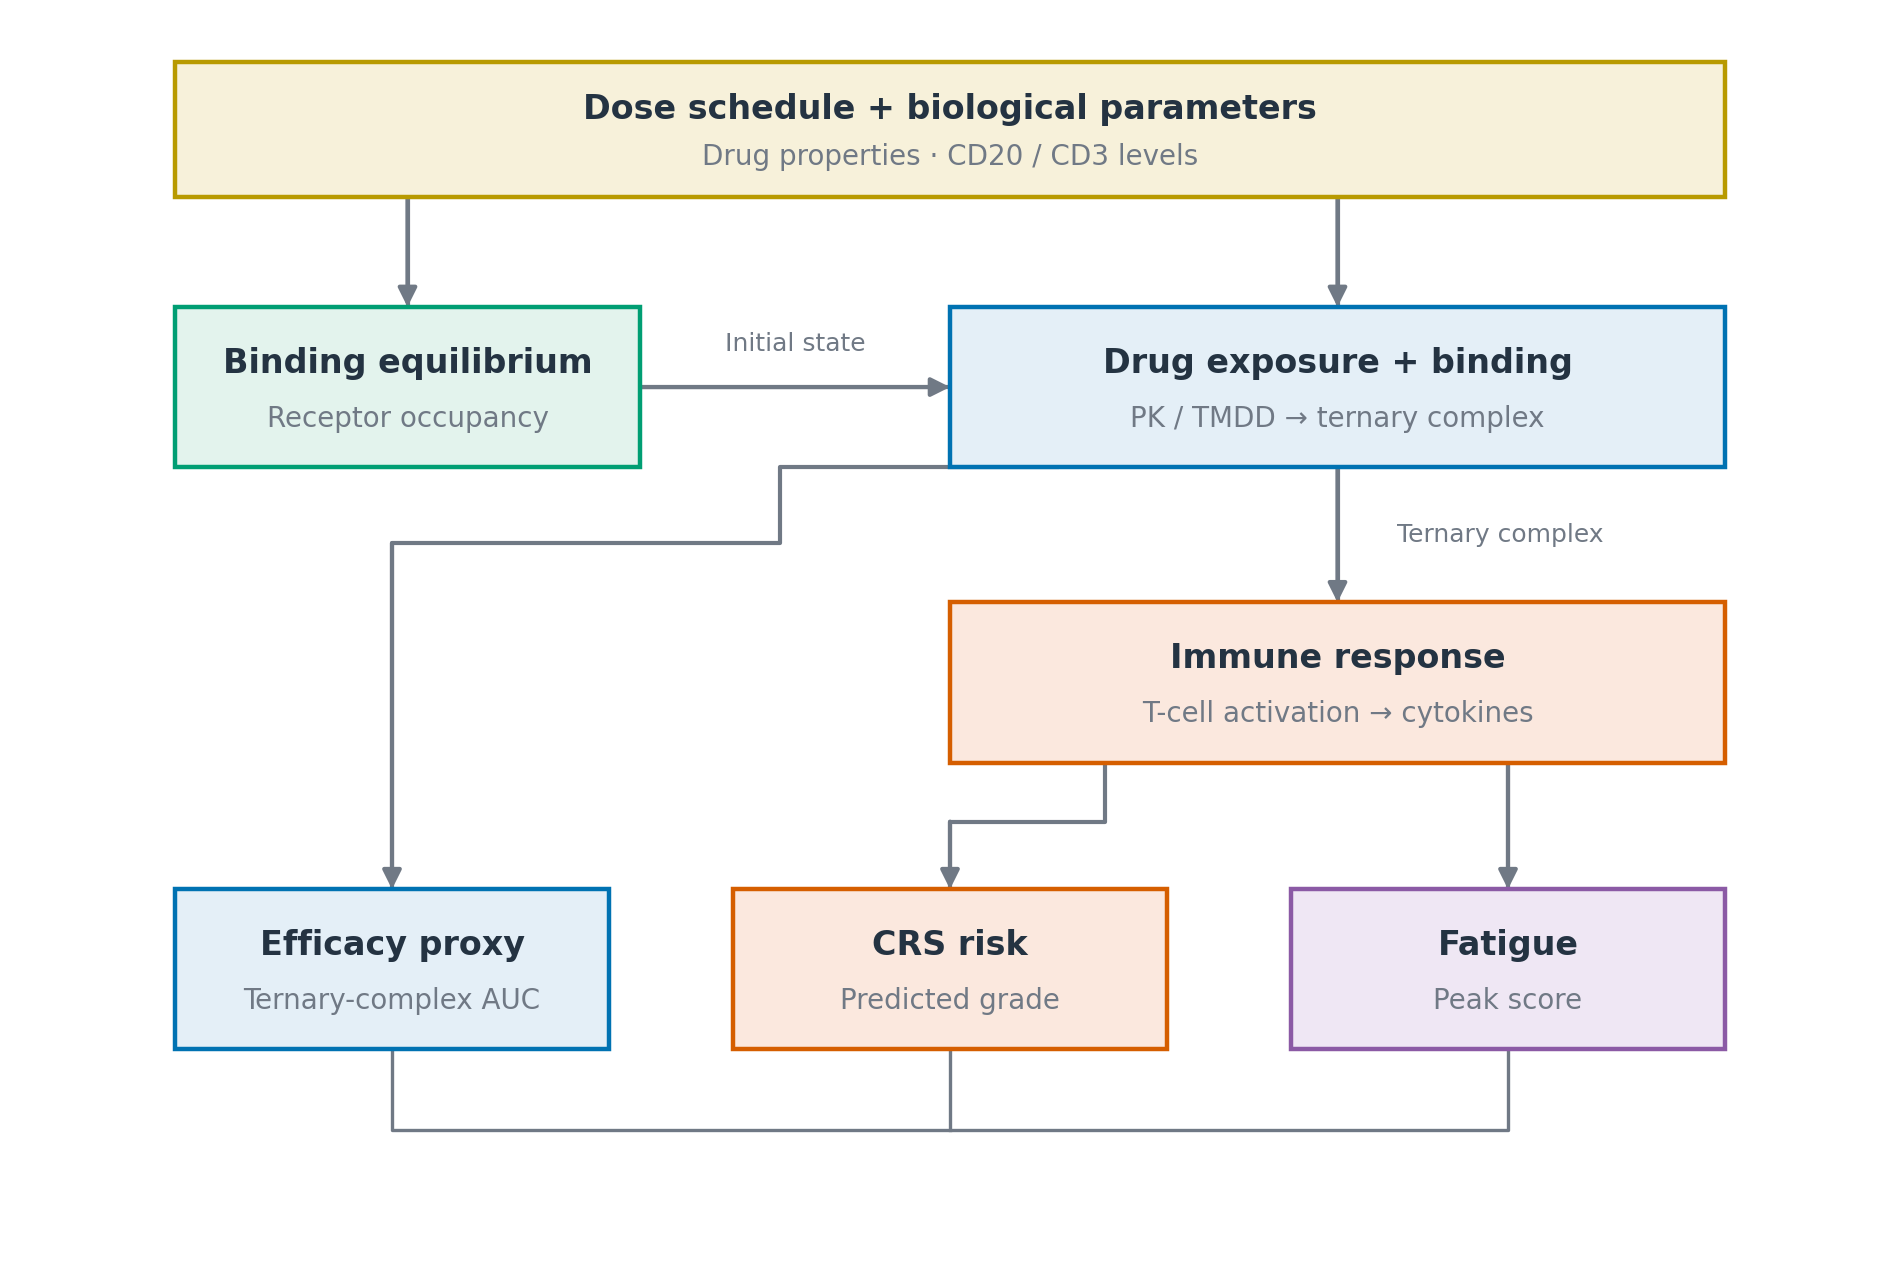
\includegraphics[width=\linewidth,height=.65\textheight,keepaspectratio]{figures/diagram_architecture.png}
\caption{Schematic of the integrated modeling framework linking drug dosing, receptor binding, and PK/TMDD dynamics to downstream cytokine release, efficacy, CRS risk, fatigue, and dose optimization.}
\label{fig:diagram-architecture}
\end{figure}

\begin{figure}[H]
\centering
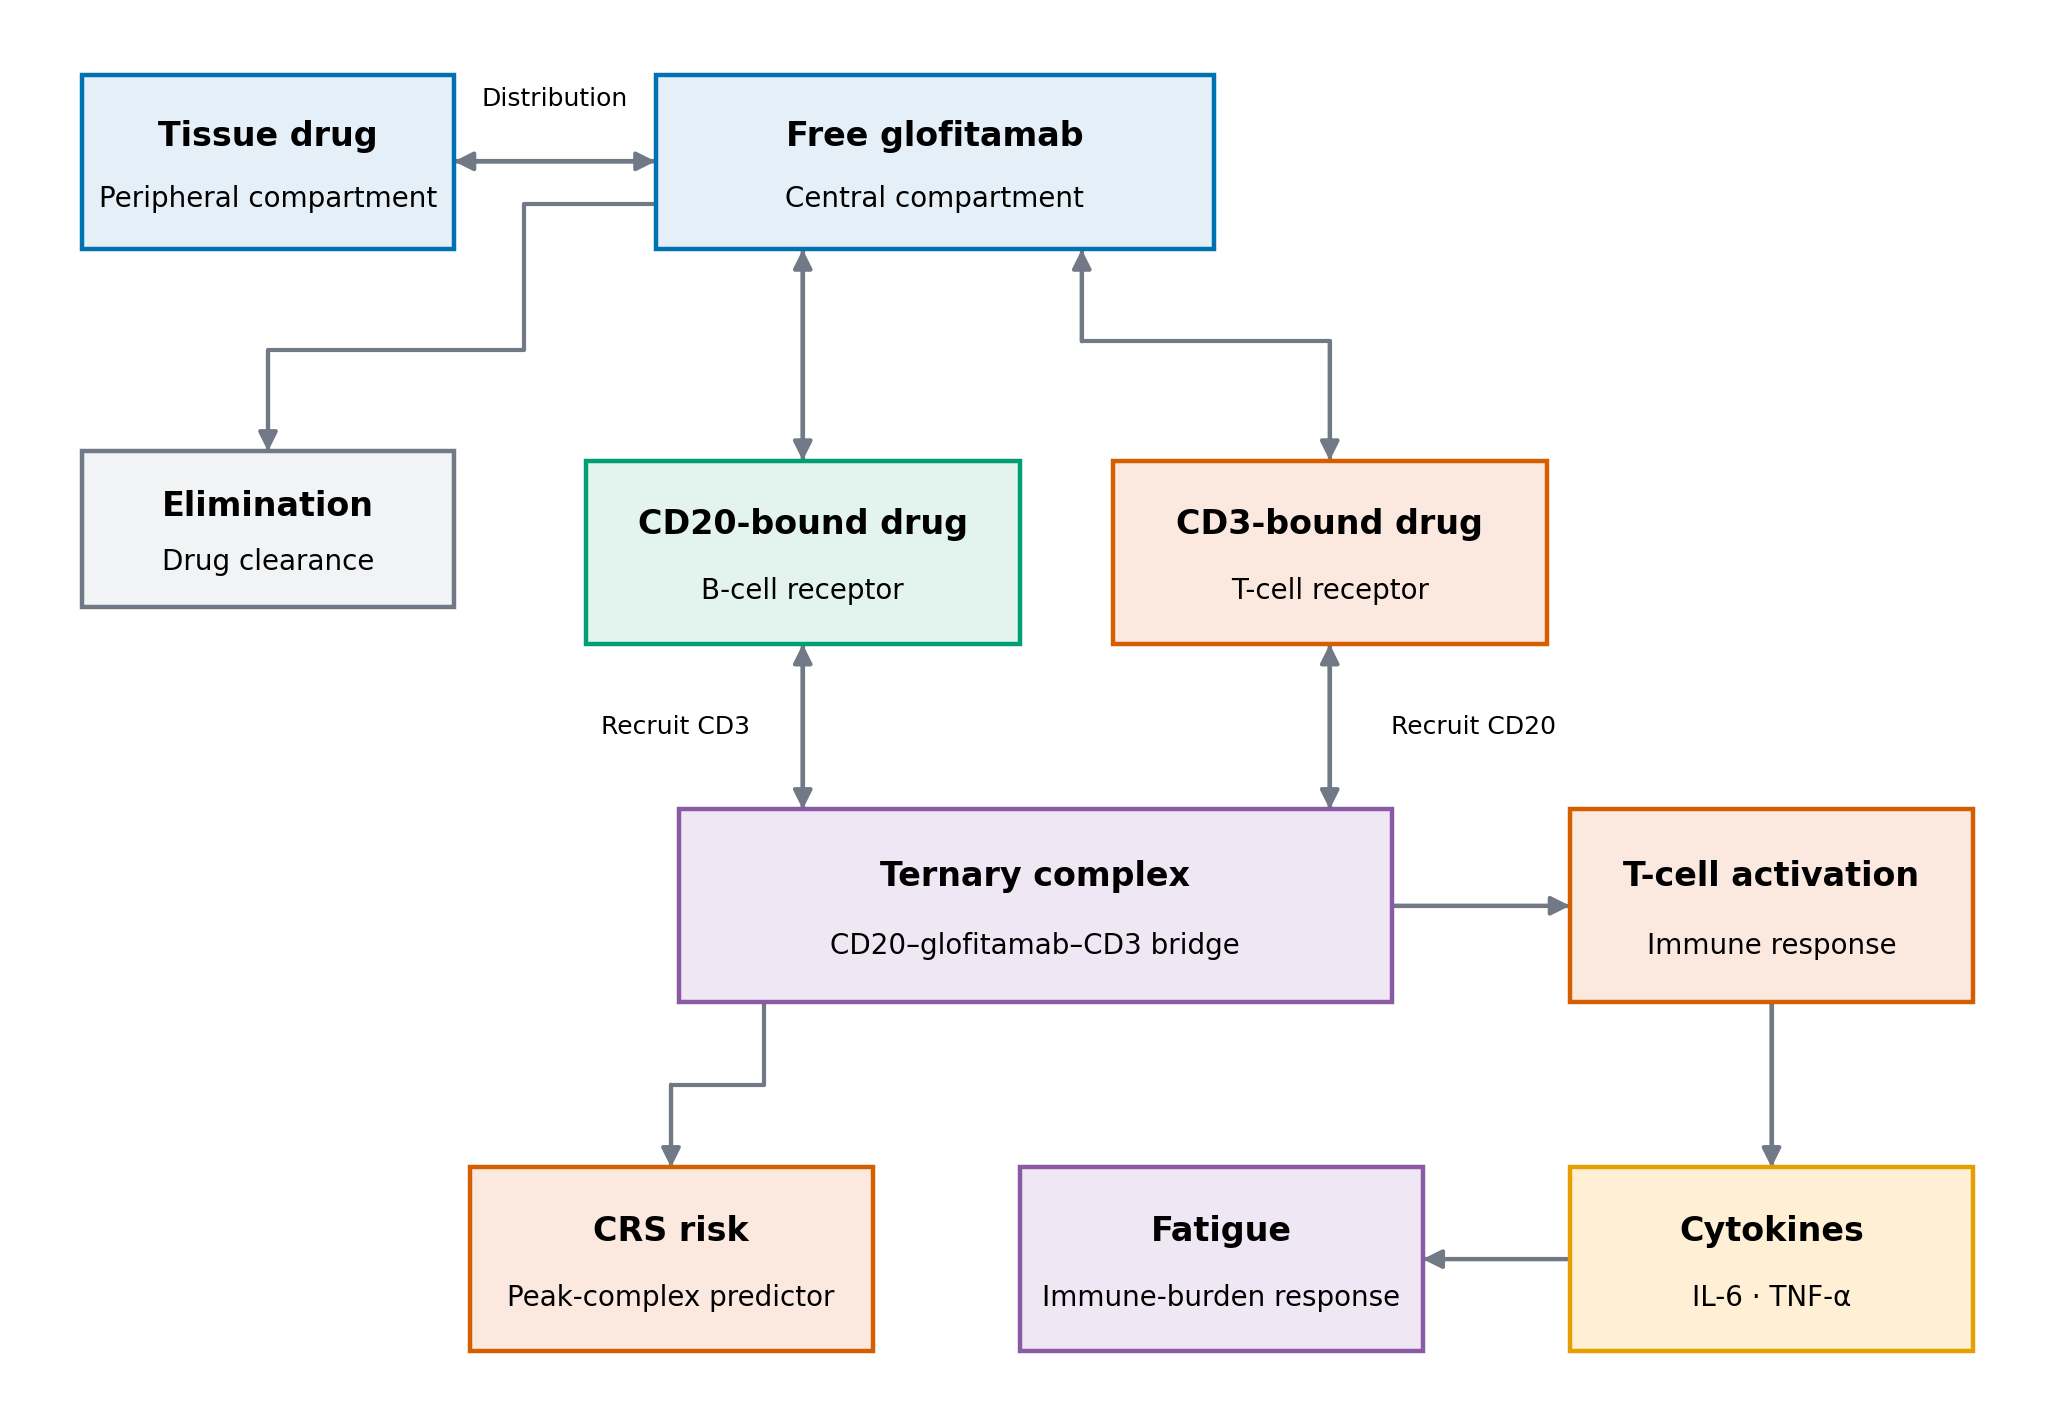
\includegraphics[width=\linewidth,height=.65\textheight,keepaspectratio]{figures/glofitamab_mechanism_of_action.png}
\caption{Schematic of the mechanistic PK/PD framework describing drug distribution, sequential CD20/CD3 binding, and formation of ternary T-cell/B-cell synapse complexes that drive T-cell activation, cytokine release, CRS severity, and fatigue outcomes.}
\label{fig:glofitamab-mechanism-of-action}
\end{figure}

\subsection{Cytokine-PK/PD Coupled Modeling Framework}

From a modeling standpoint, CRS reflects the fact that different biological processes occur on different timescales. Binding and ternary complex formation happen quickly (within minutes to hours), while pharmacokinetics, such as drug distribution and clearance, occur more slowly (over days). Because of this, many models assume quasi-equilibrium binding, where receptor interactions are treated as fast compared to PK processors [6]. Cytokine production is then modeled as a nonlinear function of the ternary complex, while cytokine  clearance is typically first-order.
\par\medskip

% Original web expression: dIL6dt = kprod ( 1+RTCEC50 + $R_{TC}$ ) - kclear IL6
\begin{equation}
\begin{aligned}
\frac{d\mathrm{IL6}}{dt}=k_{\mathrm{prod}}\left(1+\frac{R_{TC}}{EC_{50}+R_{TC}}\right)-k_{\mathrm{clear}}\mathrm{IL6}.
\end{aligned}
\label{eq:il6-response}
\end{equation}

\emph{Simplified $R_{TC}$-modulated IL-6 model based on a Hill-type cytokine framework from Lefévre et al. [18]}
\par\medskip

In Equation~\ref{eq:il6-response}, IL-6 represents the concentration of IL-6 in the bloodstream. The parameter k\textsubscript{prod} is the maximum rate at which activated immune cells produce IL-6, while $R_{TC}$ represents the concentration of the ternary complex responsible for activating T cells. The term EC\textsubscript{50} is the amount of ternary complex required to reach half of the maximum cytokine production rate, which introduces a nonlinear response. Finally, k\textsubscript{clear} represents the rate at which IL-6 is removed from circulation. Together, Equation~\ref{eq:il6-response} reflects how cytokine production increases with immune activation but eventually saturates, while clearance continuously reduces cytokine levels.
\par\medskip

To connect cytokine dynamics with drug behavior in the body, this model is coupled with pharmacokinetic equations [4, 6]. The drug concentration in the central compartment (blood plasma), denoted $D_c$, can be modeled as:
\par\medskip

\begin{equation}
\begin{aligned}
\frac{dD_c}{dt}=-\frac{CL}{V_c}D_c-k_{12}D_c+k_{21}D_p+u(t).
\end{aligned}
\label{eq:central-pk}
\end{equation}

In Equation~\ref{eq:central-pk}, CL represents the clearance rate of the drug from the body, and Vc is the volume of the central compartment. The ratio CL/V\textsubscript{c  }determines how quickly the drug concentration decreases due to elimination. The terms k\textsubscript{21  }and k\textsubscript{12  }represent the rates of drug movement between the central compartment and the tissue compartment, with D\textsubscript{p} denoting the drug concentration in the tissue compartment. The term u(t) accounts for drug input from infusion or injection.
\par\medskip

The tissue compartment is described by:
\par\medskip

\begin{equation}
\begin{aligned}
\frac{dD_p}{dt}=k_{12}D_c-k_{21}D_p.
\end{aligned}
\label{eq:peripheral-pk}
\end{equation}

Equation~\ref{eq:peripheral-pk} captures the exchange of drugs between blood and tissue, where k\textsubscript{12  }moves drugs into tissues and k\textsubscript{21} returns it to circulation.
\par\medskip

Tumor dynamics are also included to reflect how the therapy affects cancer cells:
\par\medskip

\begin{equation}
\begin{aligned}
\frac{dT_c}{dt}=rT_c-k_{\mathrm{kill}}R_{TC}.
\end{aligned}
\label{eq:tumor-growth}
\end{equation}

In Equation~\ref{eq:tumor-growth}, T represents the tumor cell population, and r is the natural tumor growth rate. The term k\textsubscript{kill} represents the rate at which activated T cells kill tumor cells, which depends on the presence of the ternary complex $R_{TC}$.
\par\medskip

% Original flattened Substack expression: $R_{TC}$ = Dc R TaKD
\begin{equation}
R_{TC}=\frac{D_c R T_a}{K_D}.
\label{eq:ternary-qe}
\end{equation}
\par\medskip

Equation~\ref{eq:ternary-qe} models the ternary complex itself.
\par\medskip

In Equation~\ref{eq:ternary-qe}, $D_c$ is the drug concentration, $R$ is the concentration of T-cell receptors, and $T_a$ represents tumor antigen concentration. The parameter $K_D$ is the binding affinity constant, which determines how strongly the drug binds to its targets. This relationship reflects how ternary complex formation increases with drug, receptor, and tumor concentration, but is limited by binding affinity.
\par\medskip

Together, Equation~\ref{eq:il6-response} through Equation~\ref{eq:ternary-qe} form a mechanistic PK/PD framework that connects drug dosing, immune activation, cytokine release, and tumor response. Previous modeling studies of bispecific antibodies support this structure, showing that multivalent binding and ternary complex formation are central drivers of therapeutic effects.
\par\medskip

\subsection{Modeling CRS and Hypothalamic Temperature Response}

The modeling of hypothalamic temperature regulation during Glofitamab treatment follows a sequential cascade that bridges molecular immune activation with physical thermodynamic response. To accurately capture this process, we utilize a mechanistic PK/PD framework adapted from [18], which tracks the drug’s journey from blood infusion to the generation of a cytokine signal (\emph{Figure~\ref{fig:original-20})}. As Glofitamab bridges T-cells and target B-cells, it triggers the transition of naive T-cells into an activated state through a series of transit compartments. This activation eventually drives a massive burst of pyrogenic cytokines, specifically IL-6, which serves as the primary biological messenger to the central nervous system. In our model, Equation~\ref{eq:thermo-naive} and Equation~\ref{eq:thermo-il6} represent this drug-to-cytokine phase, ensuring we account for the critical transit delay observed in clinical fever onset.
\par\medskip

\begin{figure}[H]
\centering
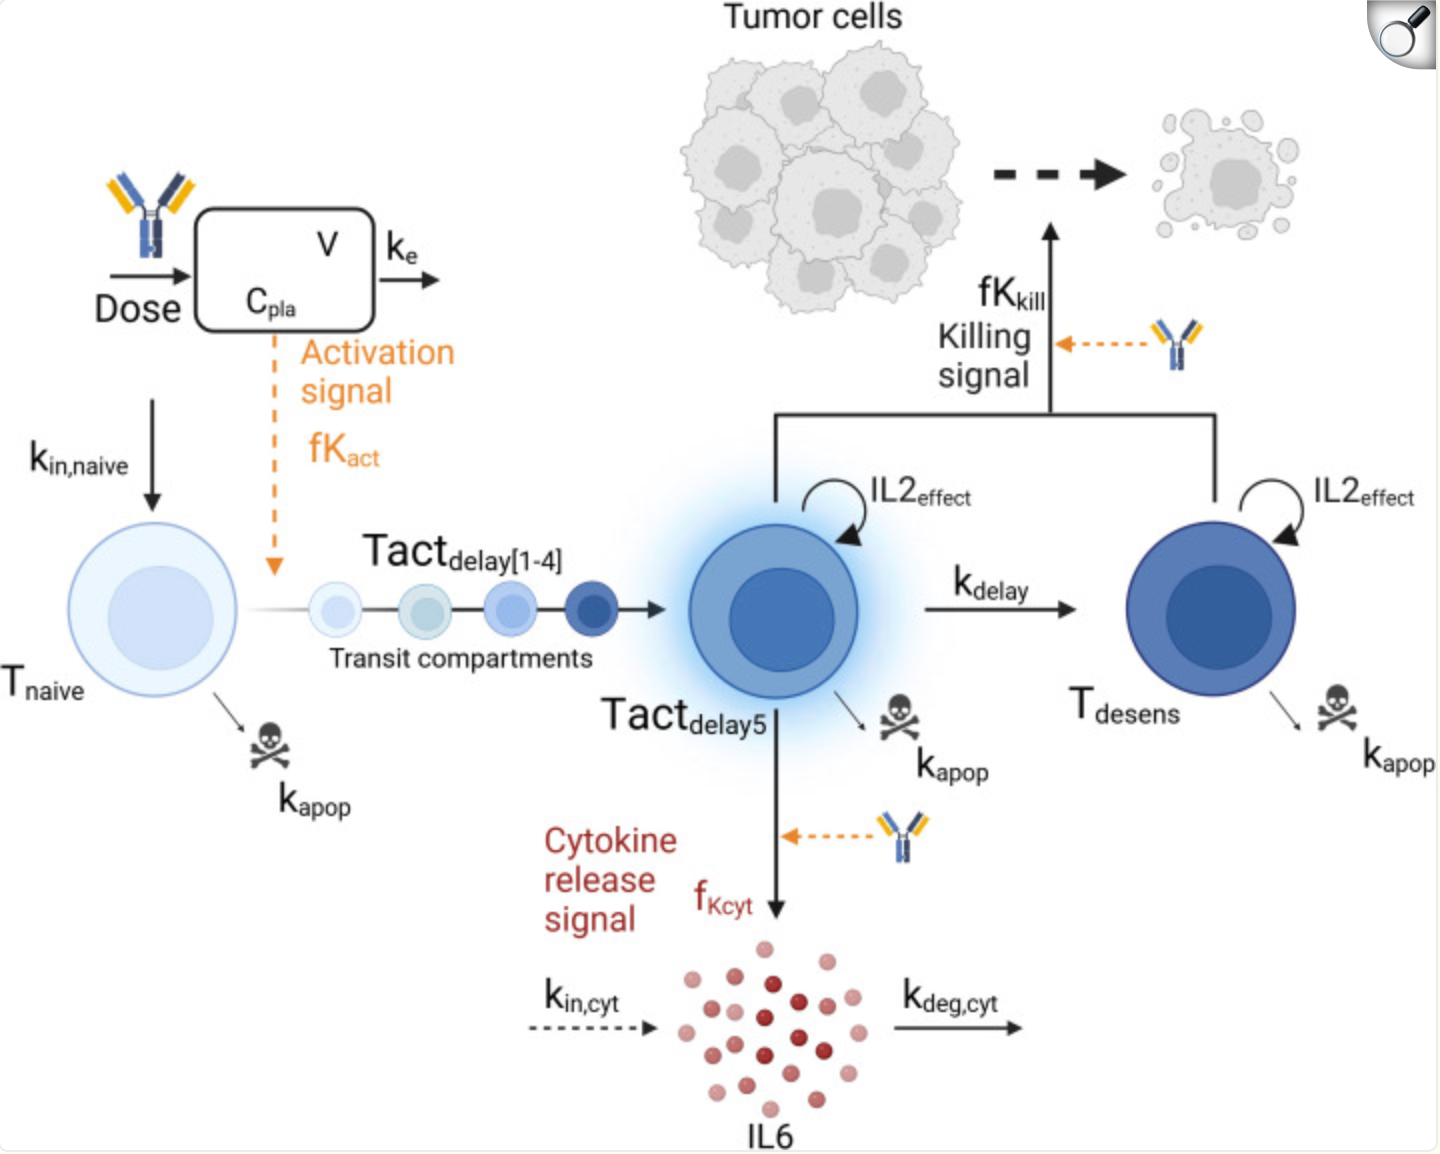
\includegraphics[width=\linewidth,height=.65\textheight,keepaspectratio]{figures/original_20.png}
\caption{Graphical representation of the mechanistic PK/PD model. The model describes the T-cell engager plasma concentration and its impact on the transition from naive T-cells to activated T-cells, leading to cytokine release and tumor cell killing [9].}
\label{fig:original-20}
\end{figure}

Since the original model in [18] concludes at the cytokine level, we expanded the architecture to include a final temperature control compartment with the corresponding ODEs (\emph{Figure~\ref{fig:original-21}}).
\par\medskip

\begin{figure}[H]
\centering

\includegraphics[width=\linewidth,height=.65\textheight,keepaspectratio]{figures/original_21.png}
\caption{Compartmental model of temperature regulation. Schematic representation of how glofitamab inputs trigger different factors such as T-cell activation and cytokine production that will then signal the hypothalamic controller to internally control the system’s temperature.}
\label{fig:original-21}
\end{figure}


\begin{equation}
\begin{aligned}
\frac{dT_{\mathrm{naive}}}{dt} &= k_1-\left(k_d+f_{k_{\mathrm{act}}}\right)T_{\mathrm{naive}}.
\end{aligned}
\label{eq:thermo-naive}
\end{equation}
\begin{equation}
\begin{aligned}
\frac{d[\mathrm{IL6}]}{dt} &= k_2\left(1+f_{k_{\mathrm{cyt}}}\right)-k_{d2}[\mathrm{IL6}].
\end{aligned}
\label{eq:thermo-il6}
\end{equation}
\begin{equation}
\begin{aligned}
T_{\mathrm{hypo}}(t) &= T_{\mathrm{base}}+\alpha\ln\left(\frac{[\mathrm{IL6}]_{\mathrm{tot}}}{[\mathrm{IL6}]_{\mathrm{base}}}\right).
\end{aligned}
\label{eq:thermo-setpoint}
\end{equation}
\begin{equation}
\begin{aligned}
\frac{dT_{\mathrm{body}}}{dt} &= k_3\left(T_{\mathrm{hypo}}-T_{\mathrm{body}}\right)-k_{d3}\left(T_{\mathrm{body}}-T_{\mathrm{room}}\right).
\end{aligned}
\label{eq:thermo-body}
\end{equation}

\emph{Equation~\ref{eq:thermo-naive} through Equation~\ref{eq:thermo-body} describe T-cell activation, IL-6 production, and thermoregulation, linking cytokine signaling to hypothalamic set-point changes and resulting body temperature dynamics}
\par\medskip

Equation~\ref{eq:thermo-setpoint} defines the hypothalamic set-point ($T_{\mathrm{hypo}}$), which is derived from the patient’s baseline temperature plus the logarithmic fold-change of IL-6 concentration scaled by a sensitivity factor, \ensuremath{\alpha}. This represents the brain’s “thermostat” being reset to a higher target in response to inflammation. Equation~\ref{eq:thermo-body} calculates the actual body temperature ($T_{\mathrm{body}}$) response, balancing internal heat generation against Newton’s Law of Cooling. By including the term $k_{d3}(T_{\mathrm{body}}-T_{\mathrm{room}})$, we account for the fact that the environment is typically cooler than the body; without this passive dissipation term, the model would inaccurately show heat accumulating indefinitely. This integrated approach allows us to simulate the full physiological arc of CRS, from the initial IV drip to the physical peak of a fever.
\par\medskip

\section{Results}

\subsection{Replication of Avidity Model}

\begin{figure}[H]
\centering
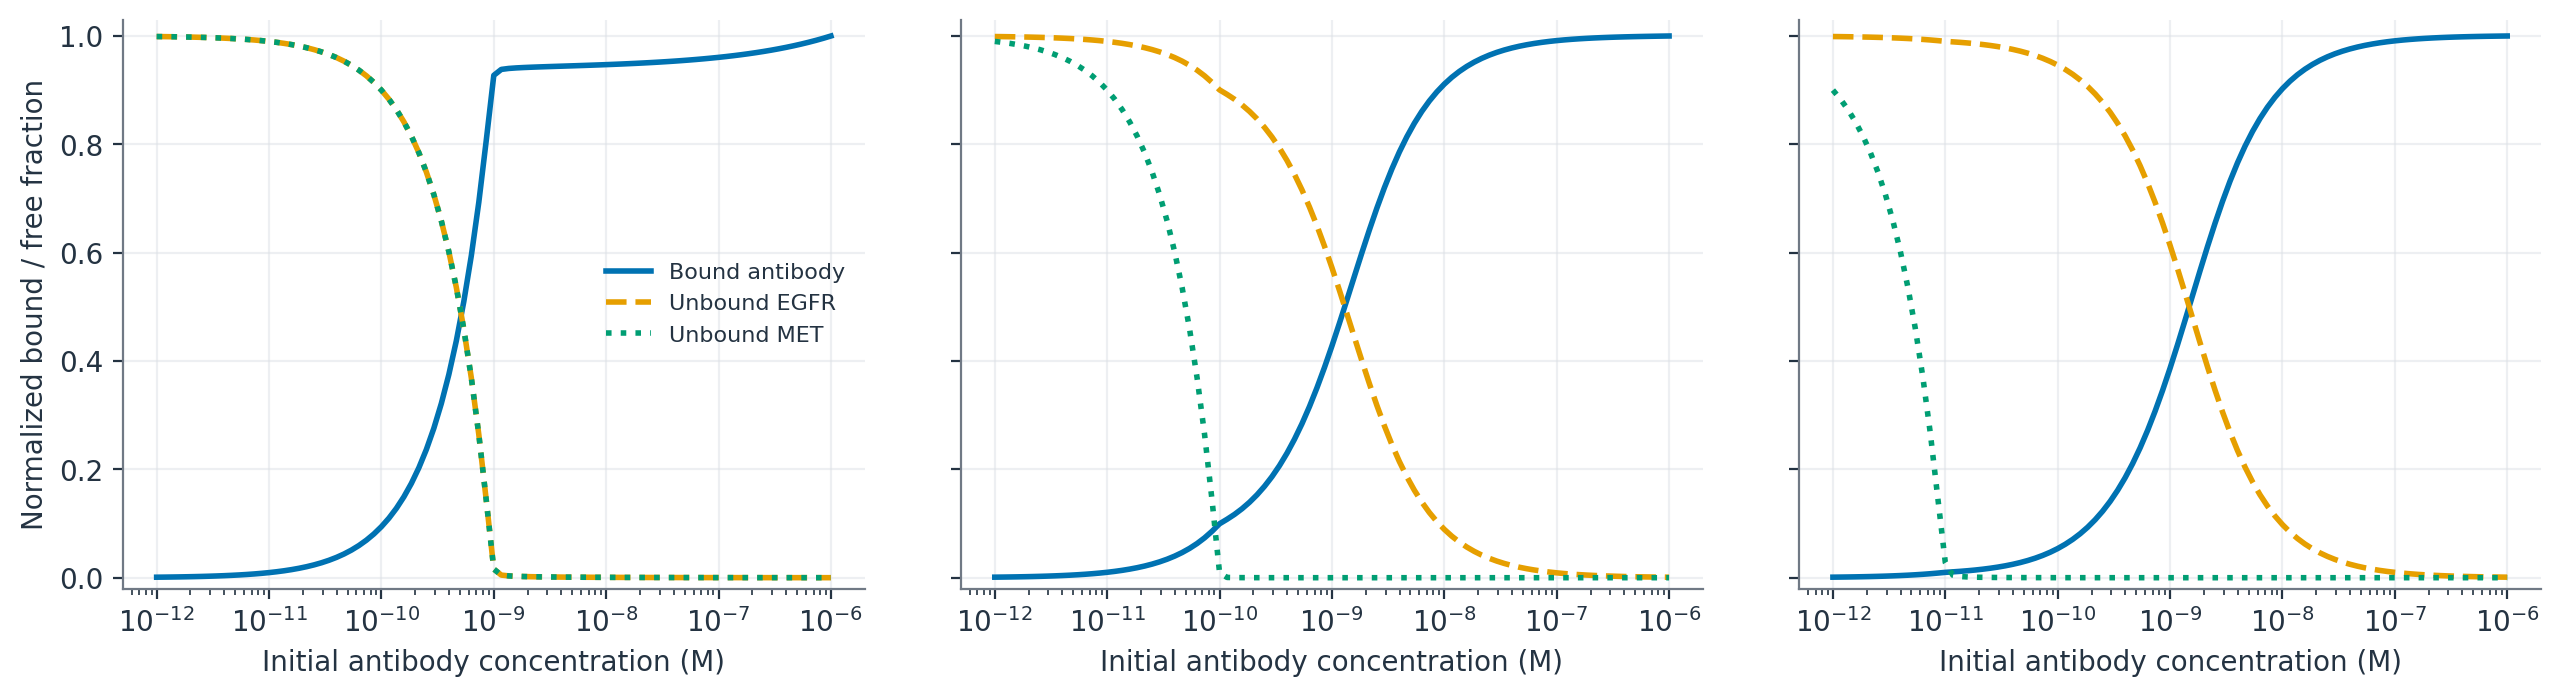
\includegraphics[width=\linewidth,height=.65\textheight,keepaspectratio]{figures/avidity_equilibrium.png}
\caption{Local steady-state reimplementation of the avidity model in Rhoden et al. [5]. Panels from left to right show EGFR:MET ratios of 1:1, 10:1, and 100:1. Bound antibody is normalized by its value at the highest sampled antibody concentration; free EGFR and MET are normalized by their own starting pools. Published baseline kinetic and geometric parameters are used. A closed antibody pool and an assumed cell density of $6.02214\times10^5$ cells/mL are used; this is not an exact reproduction of the published figure.}
\label{fig:original-23}
\end{figure}

\begin{figure}[H]
\centering
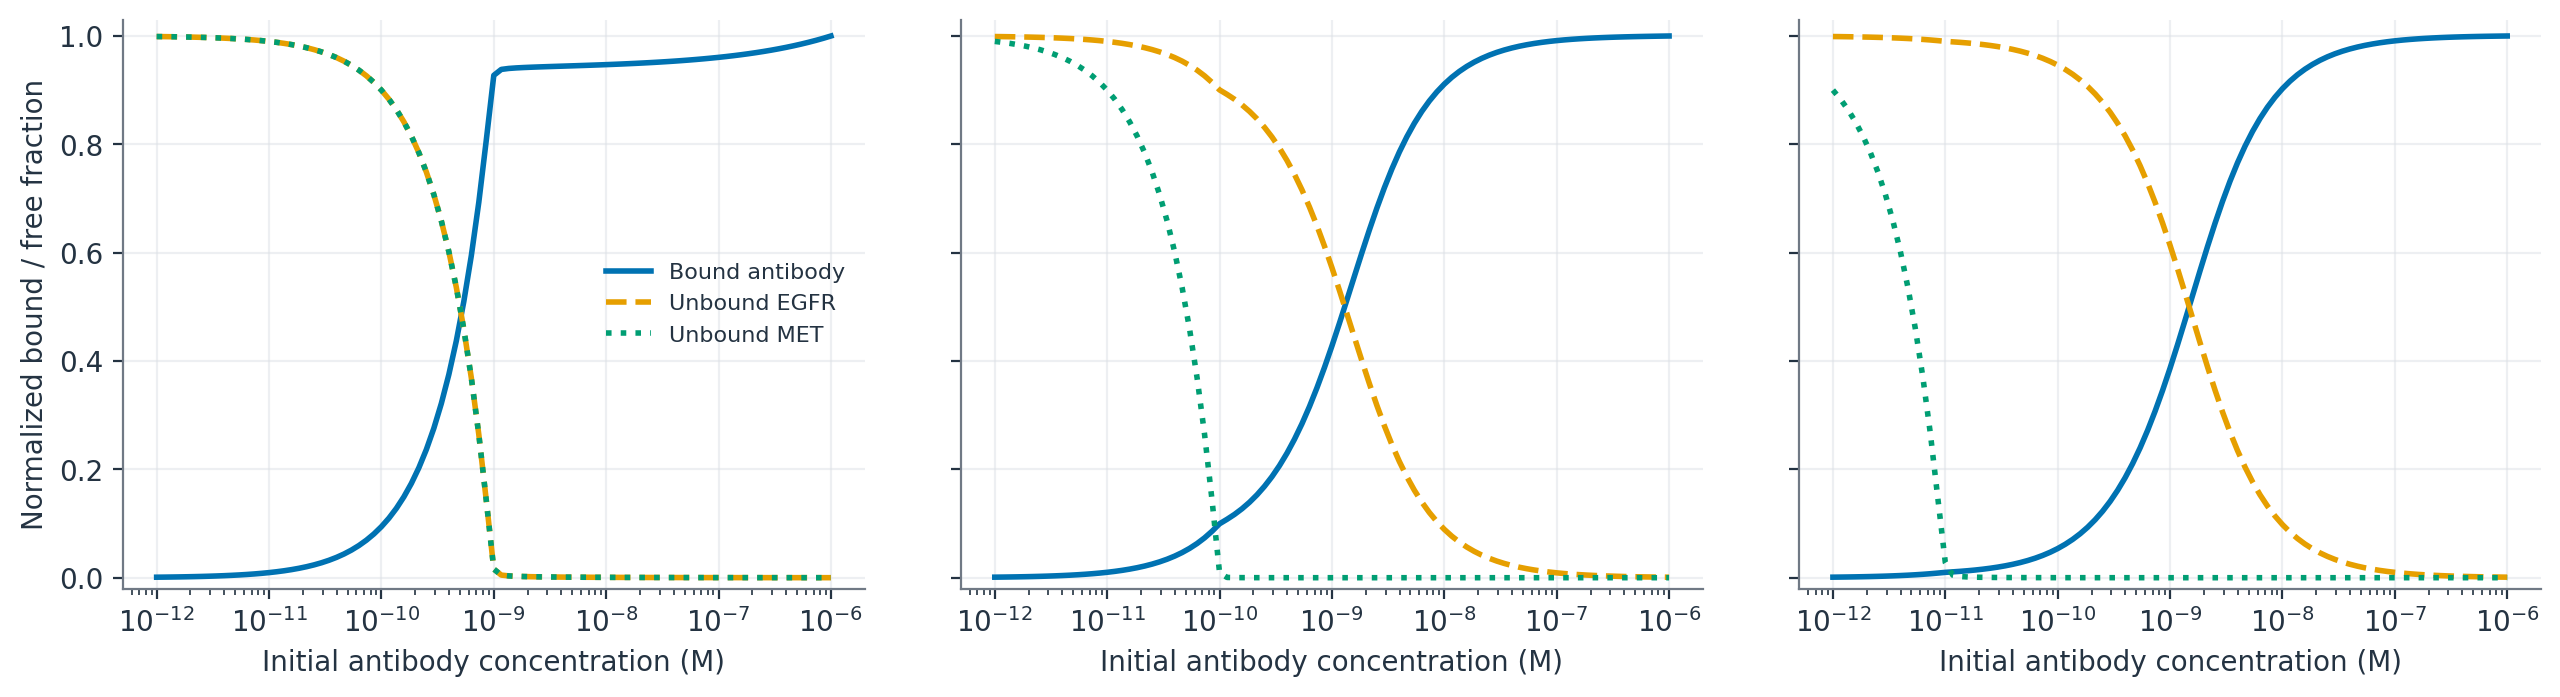
\includegraphics[width=\linewidth,height=.65\textheight,keepaspectratio]{figures/avidity_ode.png}
\caption{Independent ODE verification of Figure~\ref{fig:original-23}. The six-state mass-action model is integrated from unbound initial conditions to stationary state for each antibody concentration, using the same parameters, normalization, and panel ordering. The curves are checked against the independent algebraic solution at every dose. Numerical relaxation time is not an experimental incubation time.}
\label{fig:original-24}
\end{figure}

\subsection{Replication of BS1 Binding Model}

During the binding phase (0–2 hours), the ternary complex (IL-6R-BS1-IL-8R, orange) saturated near 3.1 × 10\textsuperscript{5} complexes/cell, mirroring the IL-6R ceiling of 3.16 × 10\textsuperscript{5} \#/cell, which confirmed IL-6R as the limiting receptor. The binary IL-8R complex (BS1-IL-8R, blue) accumulated steadily thereafter as excess antibodies engaged the more abundant IL-8R pool. The binary IL-6R complex (BS1-IL-6R, yellow) remained near zero throughout, as any IL-6R-bound antibody rapidly completed cross-linking before a stable binary species could accumulate.
\par\medskip

Upon washout at 2 hours, the binary IL-8R complex decayed while the ternary complex exhibited a brief upward inflection before plateauing — a direct manifestation of the avidity effect, wherein dissociating binary complexes release free receptors that tethered antibodies exploit to complete cross-linking. The result is sustained ternary occupancy in the complete absence of free drug, with implications for therapeutic activity beyond the pharmacokinetic window.
\par\medskip

\begin{figure}[H]
\centering
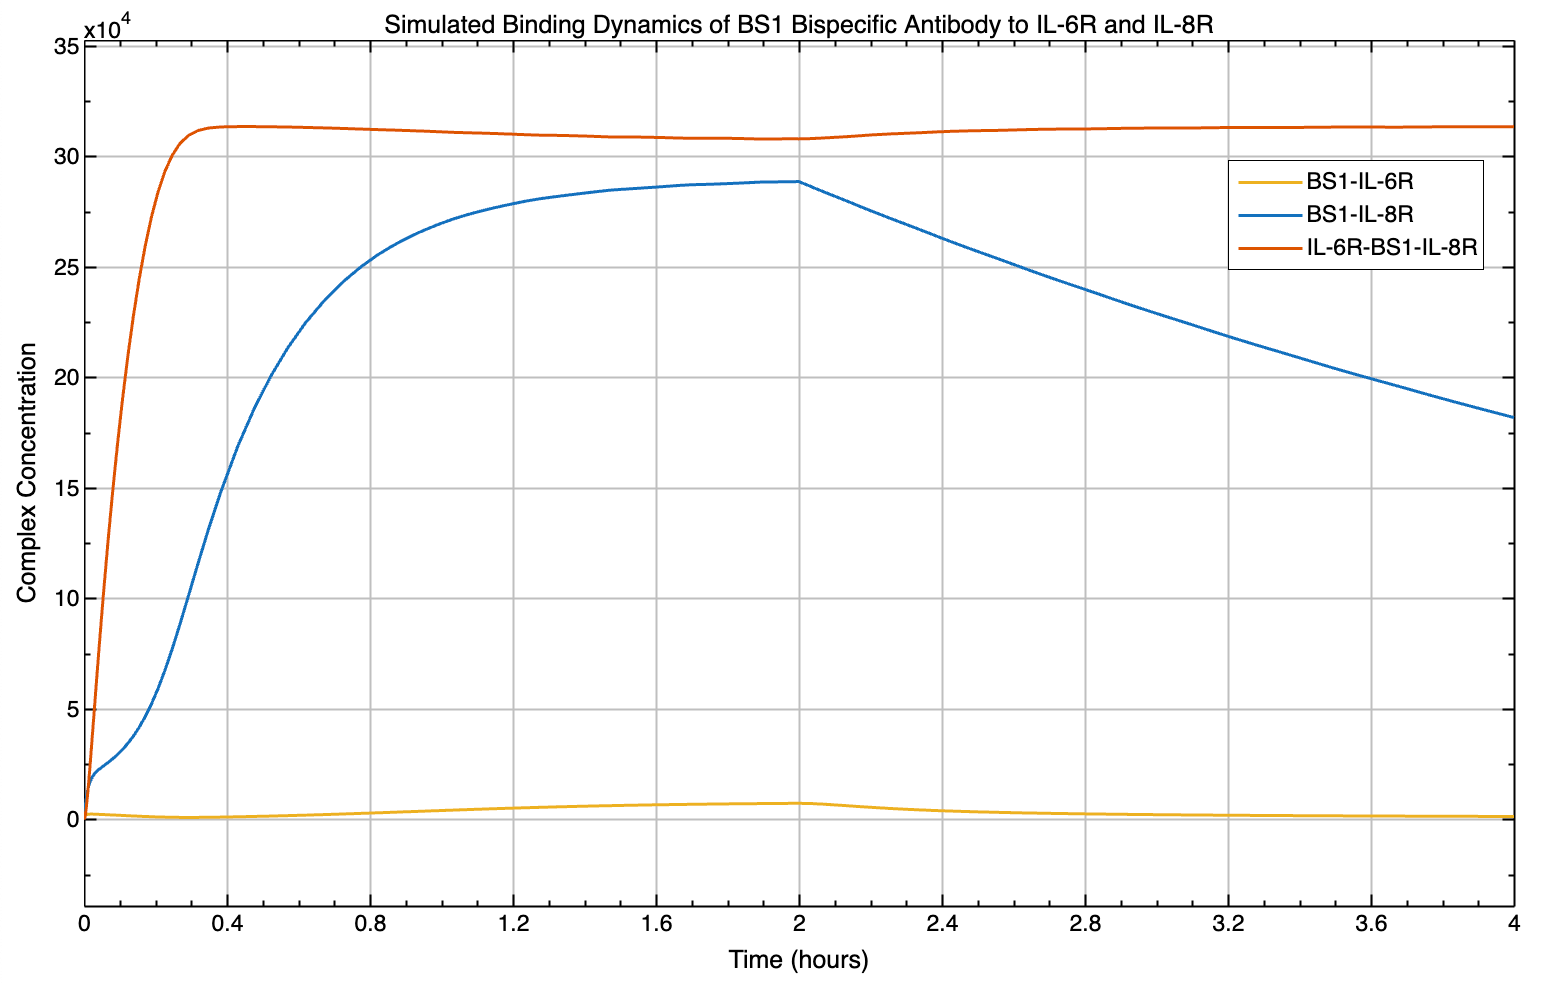
\includegraphics[width=\linewidth,height=.65\textheight,keepaspectratio]{figures/original_25.png}
\caption{Simulated binding dynamics of the BS1 bispecific antibody over 4 hours. BS1-IL-6R (yellow): binary IL-6R complex; BS1-IL-8R (blue): binary IL-8R complex; IL-6R-BS1-IL-8R (orange): ternary complex. Washout at t = 2 hours.}
\label{fig:original-25}
\end{figure}

\subsection{Dose-dependent Binding Behavior}

To extend the BS1 replication beyond the four-hour time-course shown in \emph{Figure~\ref{fig:original-25}}, we analyzed how initial BS1 concentration affected final receptor occupancy and ternary complex formation under a fixed receptor condition of IL-6R = 50 and IL-8R = 50. The simulations showed that total bound receptor increased monotonically with BS1 dose and approached saturation near the total available receptor pool, while ternary complex formation followed a bell-shaped dose-response, reaching a maximum at an intermediate concentration and declining at higher doses. This indicates that greater overall receptor occupancy does not necessarily correspond to greater productive bispecific binding. Instead, the linked two-receptor state is maximized within an intermediate dose window, while very high BS1 concentrations increasingly favor one-sided binary binding over ternary complex formation. These dose-response results complement the original BS1 time-course replication by showing that, in addition to avidity and post-washout persistence, concentration strongly shapes the balance between total target engagement and the functionally important bispecific complex. This is directly relevant to the broader Glofitamab framework, where the analogous functional objective is not simply more binding, but formation of the productive bridged state between target B-cells and effector T-cells.
\par\medskip

\begin{figure}[H]
\centering
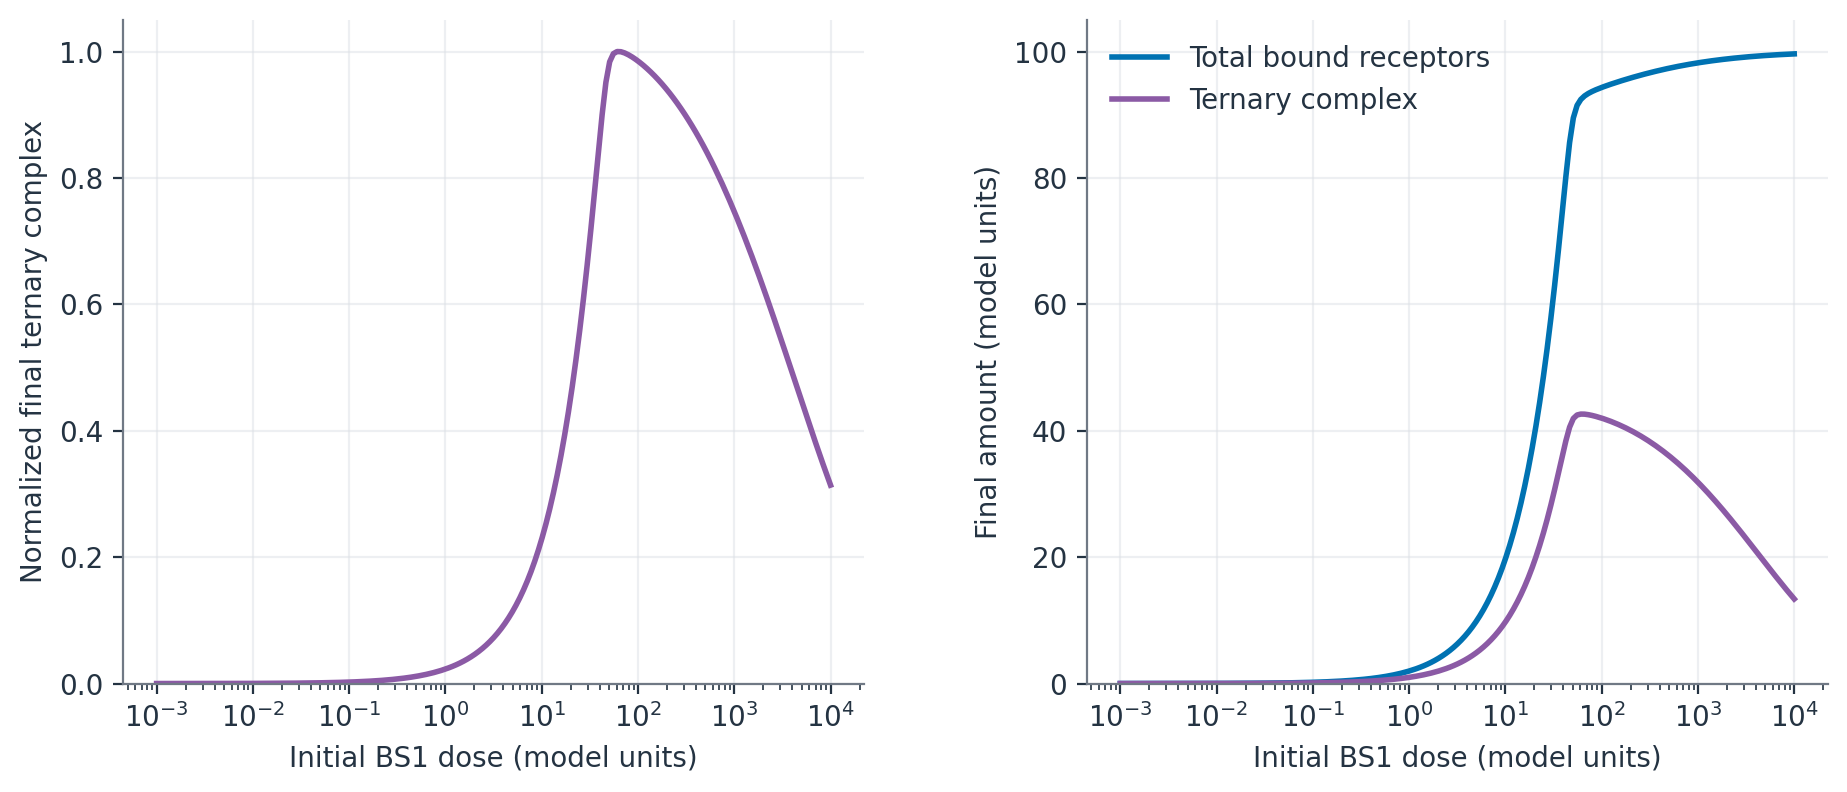
\includegraphics[width=\linewidth,height=.65\textheight,keepaspectratio]{figures/bs1_dose_response_combined.png}
\caption{Reconstructed BS1 dose response for initial IL-6R and IL-8R pools of 50 each. Left: final ternary complex normalized by its maximum over the dose grid. Right: total occupied receptors (binary complexes plus twice the ternary complex) and absolute ternary complex. Each dose is integrated for an assumed 14,400 seconds without washout. Rate constants are recovered from the available Simulink binding block, which labels them Glofitamab estimates; the original sweep settings are unavailable. These calculations reproduce the qualitative binding pattern, not the numerical values in the original screenshots.}
\label{fig:bs1-dose-response-combined}
\end{figure}

\subsection{Glofitamab Binding Dynamics (2:1 Architecture)}

During the binding phase (0–2 hours), the high-affinity CD20 arms drove rapid B-cell coating: the monovalent B-cell complex (yellow) peaked near 8.7 × 10\textsuperscript{4}, and the bivalent anchor (blue) stabilized near 4.8 × 10\textsuperscript{4} with notably flat kinetics once formed. The monovalent T-cell complex (orange) also accumulated given the 100 nM dose exceeding the CD3 K\_d, but these represent transient solution-phase contacts rather than productive synaptic events. Accordingly, the fully locked synapse (purple) remained low throughout the infusion, rising only gradually — reflecting the geometric constraint of physically bridging two cell types and constituting the key safety mechanism limiting acute T-cell hyperactivation.
\par\medskip

Upon washout at 2 hours, the monovalent T-cell complex (orange) decayed sharply while the bivalent CD20 anchor (blue) remained almost entirely stable — a direct consequence of cooperative bivalent binding preventing full dissociation. Strikingly, both synapse species (green and purple) continued to increase post-washout: antibodies anchored to B-cells via both CD20 arms efficiently captured CD3 receptors freed by the decay of monovalent complexes, forming additional synapses without any free drug present. This post-washout synapse growth mirrors the avidity effect observed in the BS1 model and provides a mechanistic basis for Glofitamab’s sustained anti-tumor activity beyond its pharmacokinetic window.
\par\medskip

\begin{figure}[H]
\centering
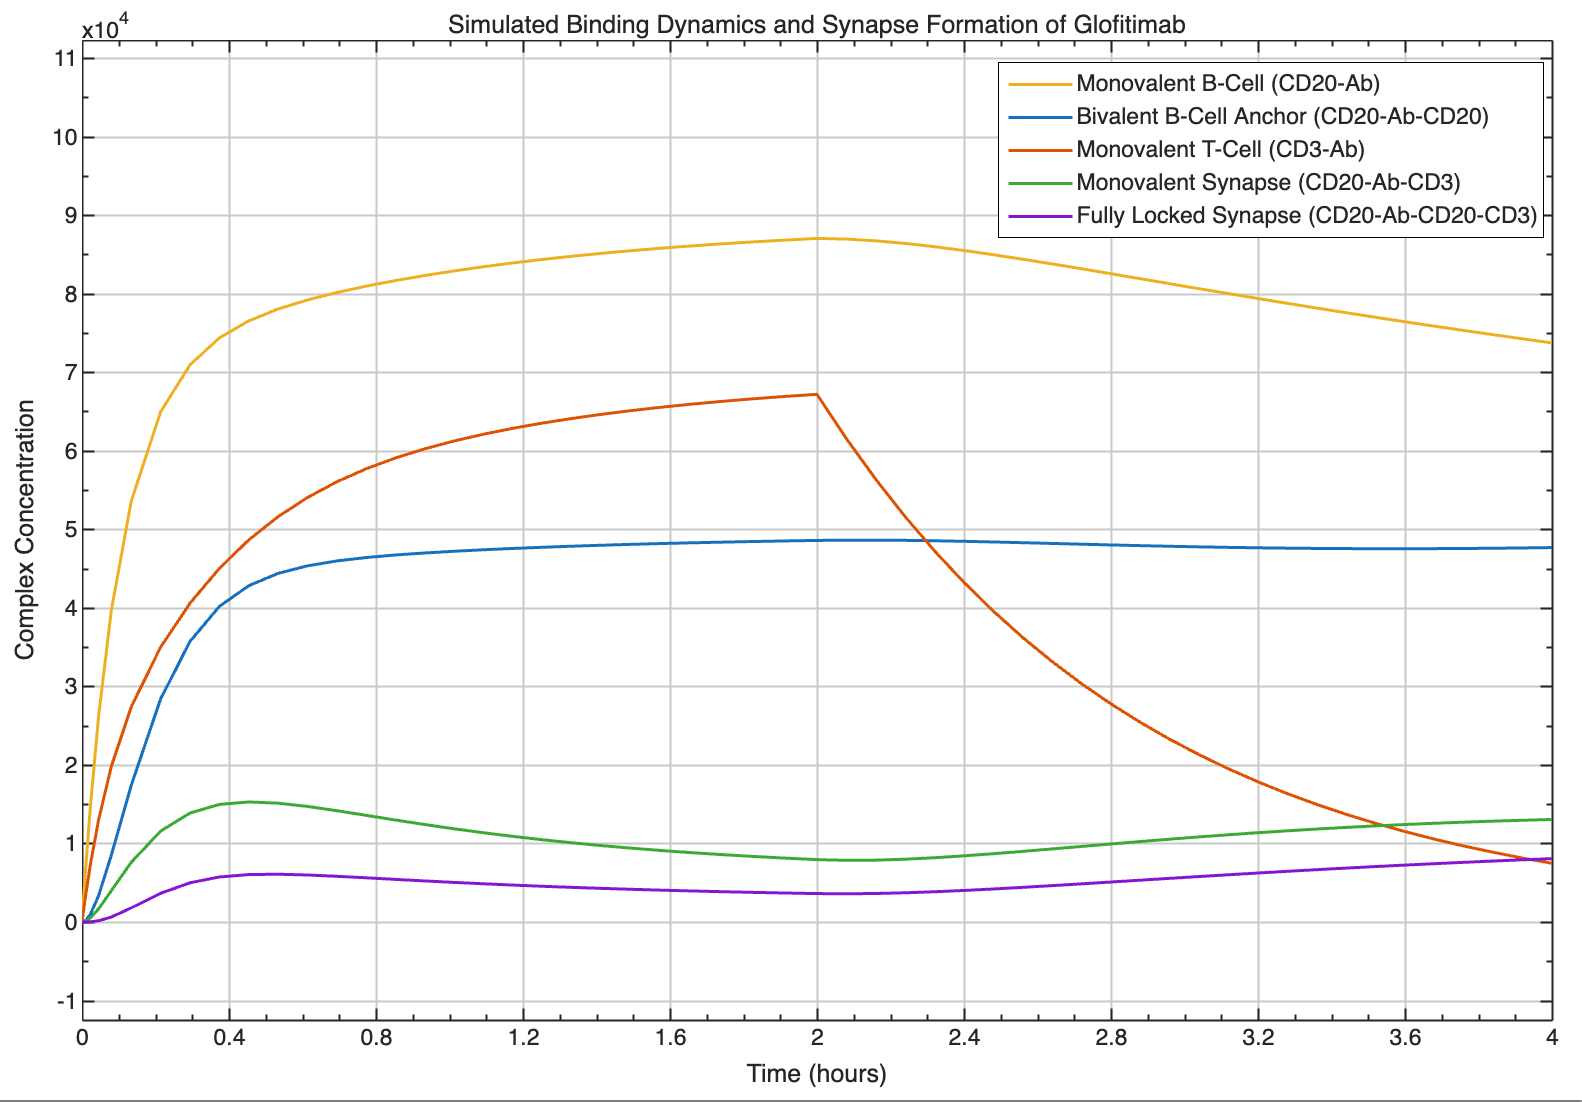
\includegraphics[width=\linewidth,height=.65\textheight,keepaspectratio]{figures/original_28.png}
\caption{Simulated binding dynamics and synapse formation for Glofitamab over 4 hours. Monovalent B-Cell (yellow); Bivalent B-Cell Anchor (blue); Monovalent T-Cell (orange); Monovalent Synapse (green); Fully Locked Synapse (purple). Washout at t = 2 hours.}
\label{fig:original-28}
\end{figure}

\subsection{Comparative Analysis of 1:1 versus 2:1 Architectures}

Both models converge on the same core finding: avidity-driven complex stabilization allows therapeutic bridging activity to outlast free drug availability, with the highest-order complexes increasing post-washout as weaker monovalent species break apart and donate free receptors.
\par\medskip

The 2:1 Glofitamab architecture adds two clinically meaningful refinements. First, bivalent CD20 anchoring pre-positions the antibody at the tumor site before any T-cell contact, creating a B-cell sink that concentrates activity where it is needed. Second, weak CD3 affinity gates T-cell activation on tumor co-engagement, substantially reducing systemic cytokine risk. These properties are encoded directly in the model parameters and their mechanistic consequences — sustained synapse formation and CRS mitigation — are observable in the simulation dynamics and will be explored further in the Discussion.
\par\medskip

\subsection{CRS and Dose-Dependent Dynamics}

To further investigate CRS dynamics, multiple ODE-based models were integrated, including the CRS framework and hypothalamic regulation components described earlier. The results of these simulations are presented below, with full parameter tables provided.
\par\medskip

\begin{figure}[H]
\centering
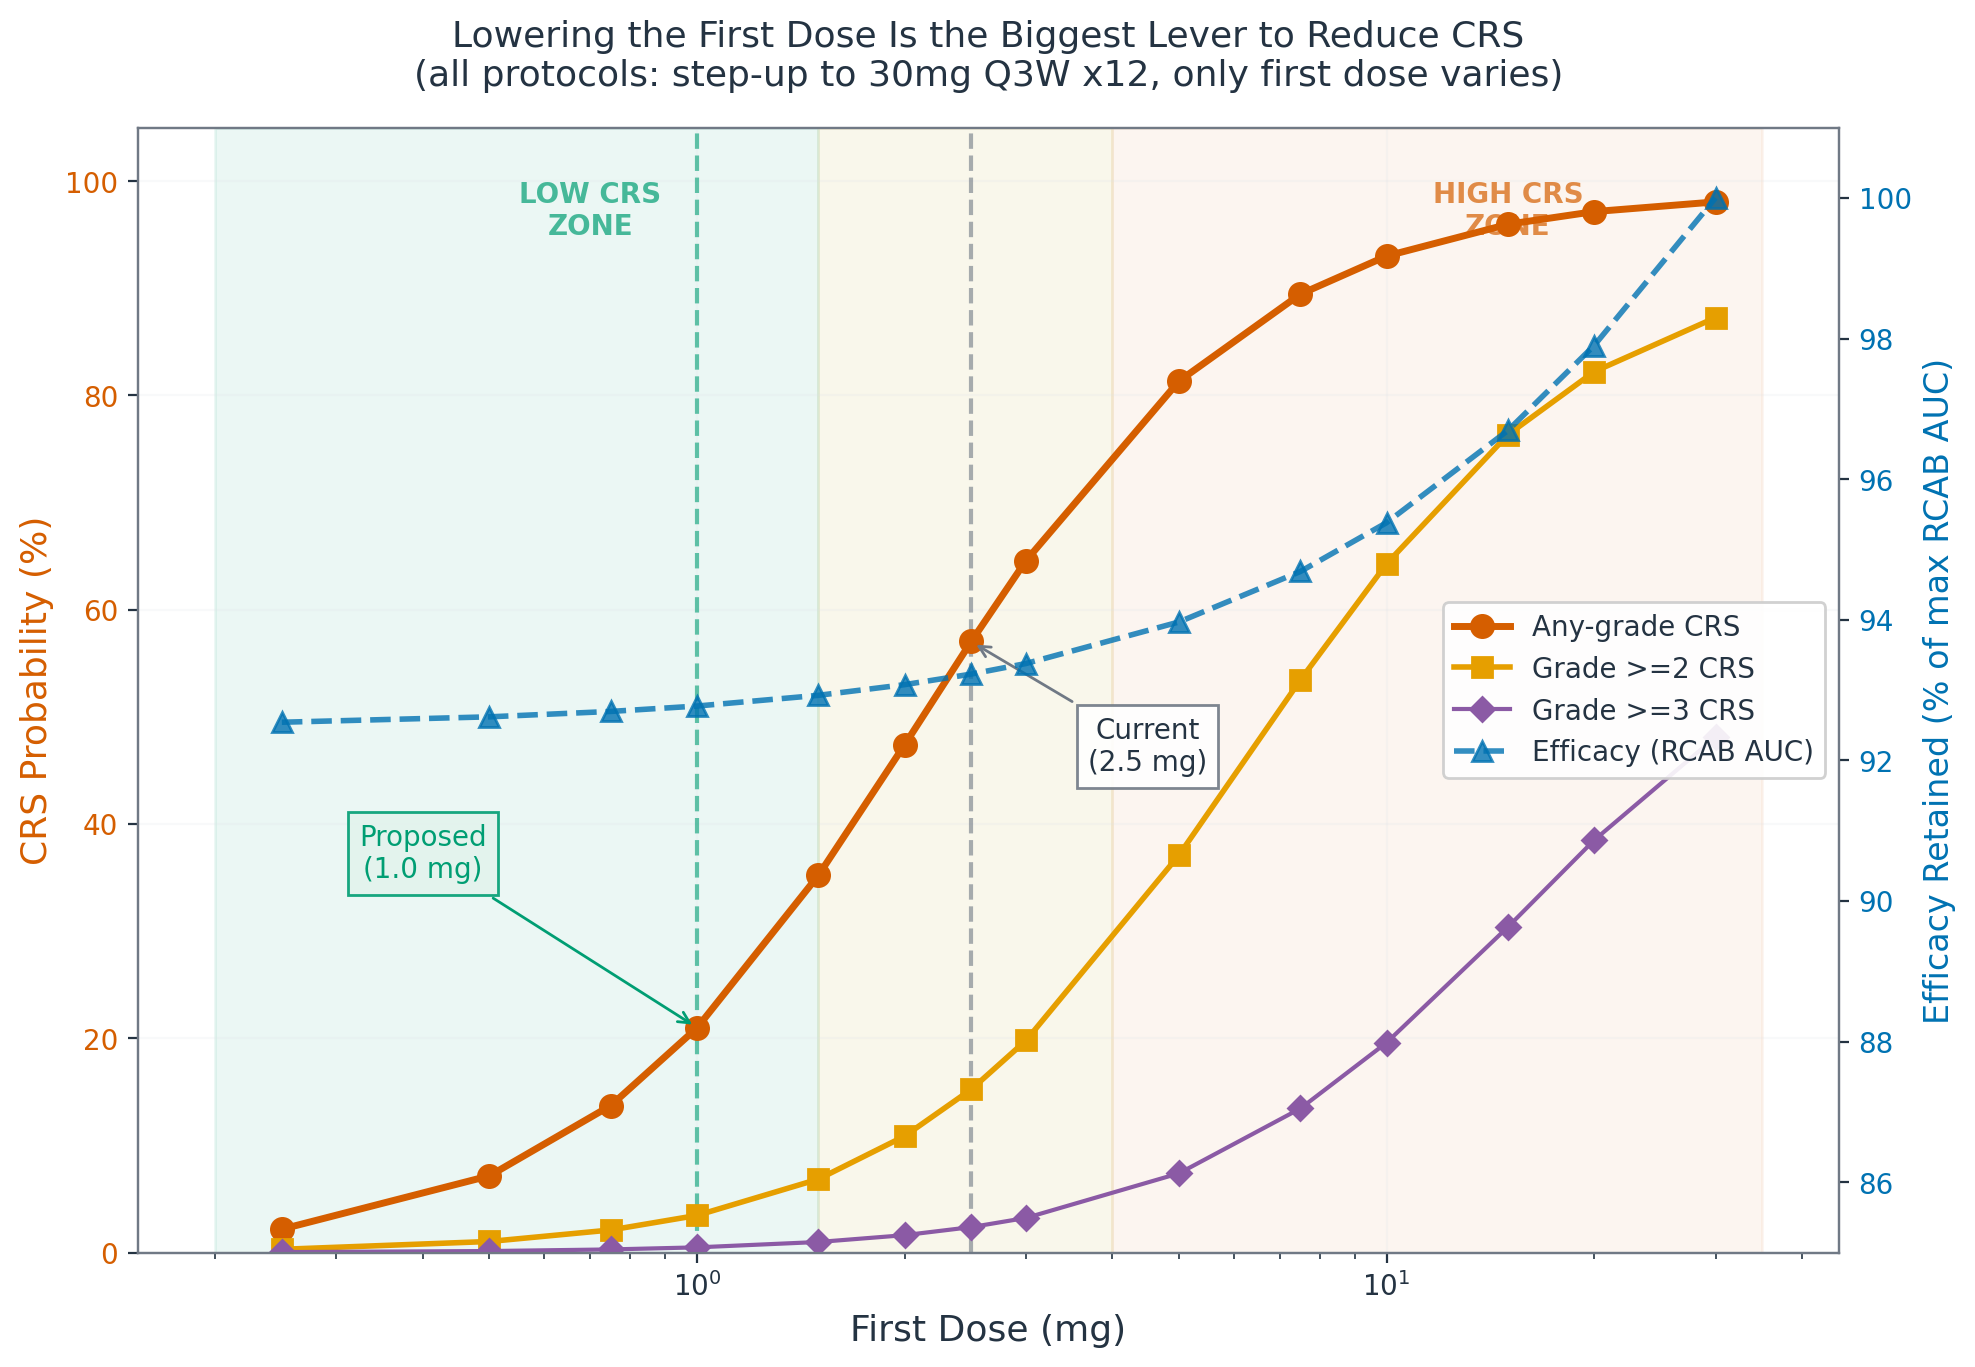
\includegraphics[width=\linewidth,height=.65\textheight,keepaspectratio]{figures/fig1_first_dose_sweet_spot.png}
\caption{CRS probability plotted against first dose size. This figure shows the effect of the first-dose on CRS risk and efficacy in a system. Lower initial doses reduces the chance of CRS and preserves efficacy as well (RCAB AUC).}
\label{fig:fig1-first-dose-sweet-spot}
\end{figure}

 Lowering the initial dose significantly reduces the probability of CRS, including both moderate (grade 2) and severe (grade 3) cases, as well as overall incidence. This supports the idea that early immune activation is highly sensitive to initial dosing conditions.
\par\medskip

\begin{figure}[H]
\centering
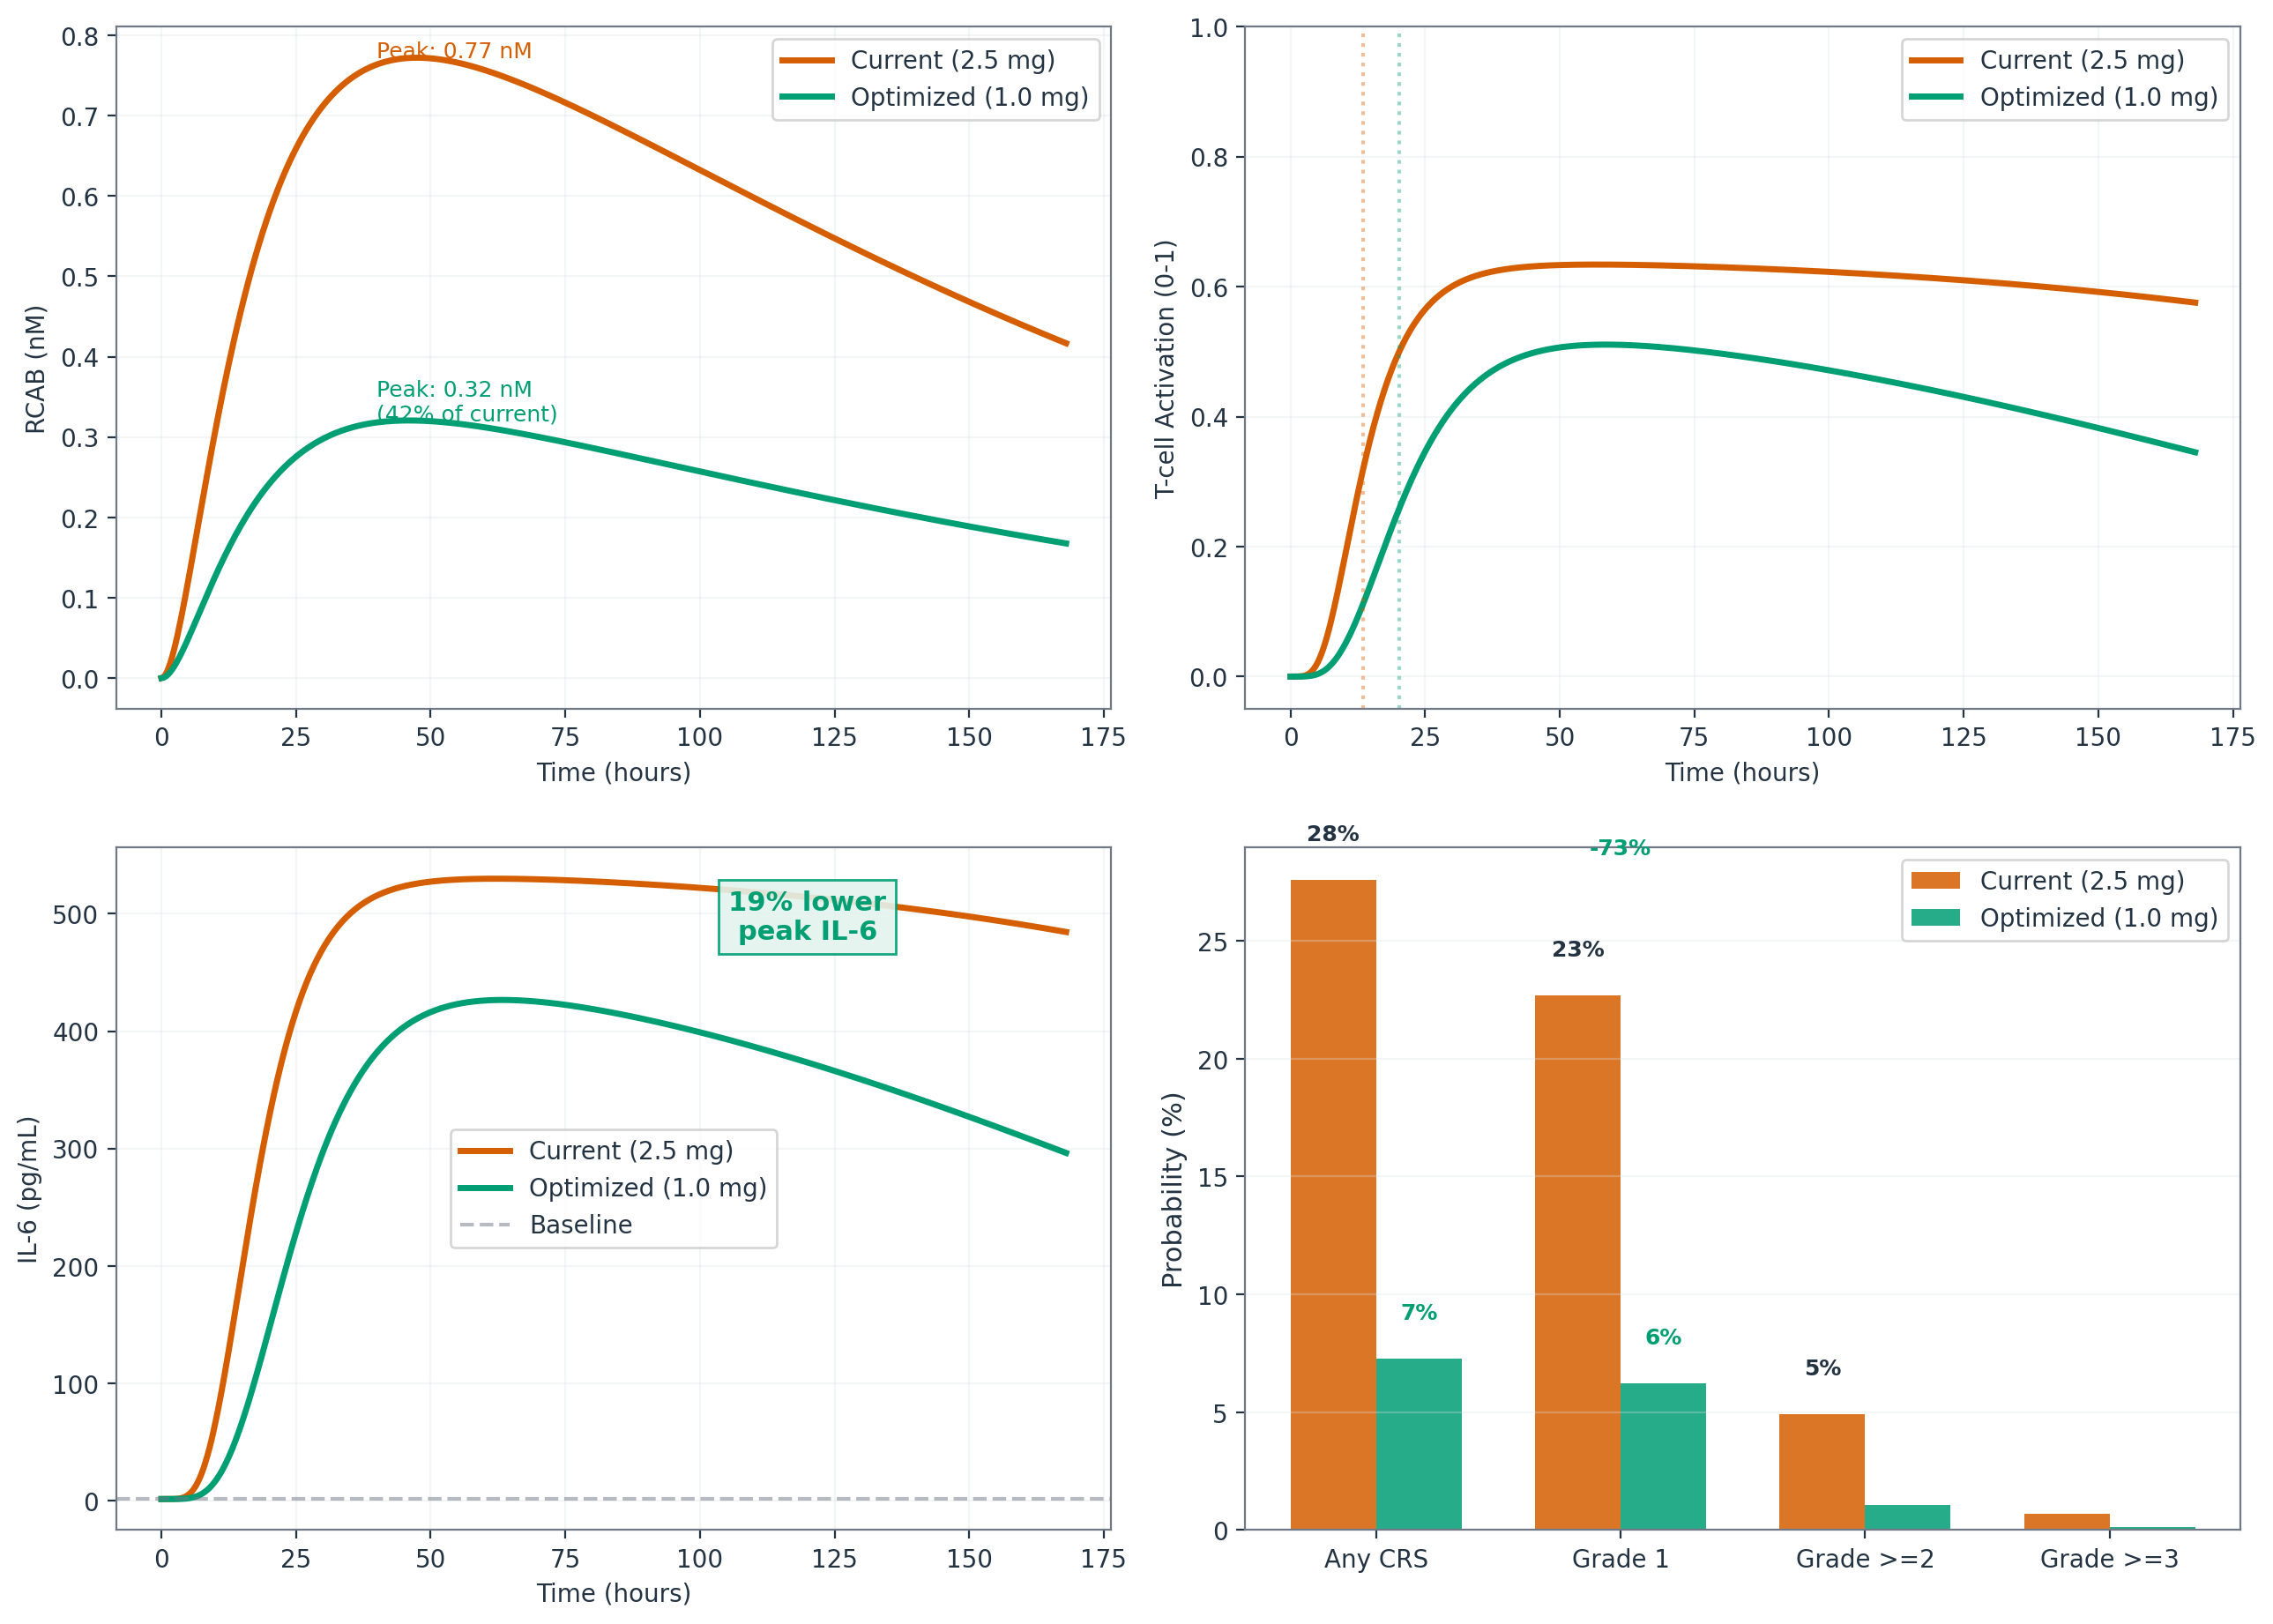
\includegraphics[width=\linewidth,height=.65\textheight,keepaspectratio]{figures/fig2_current_vs_optimized.png}
\caption{Complex formation, T-Cell activation, IL-6 cytokine release, and CRS risk for a smaller first dose. Figures above show the comparison of current and optimized first doses (2.5 mg and 1.0 mg respectively) to represent the reduced values of ternary complex formation, T-cell activation, IL-6 release, and significantly lower CRS risk with the optimized first dose in comparison to the current regimen. Obinutuzumab pretreatment and the maintenance schedule are identical in both regimens.}
\label{fig:fig2-current-vs-optimized}
\end{figure}

Reducing the initial dose leads to a lower peak in ternary complex formation, which in turn limits downstream T-cell activation and cytokine release. This demonstrates that controlling early binding dynamics is an effective strategy for reducing CRS risk.
\par\medskip

\begin{figure}[H]
\centering
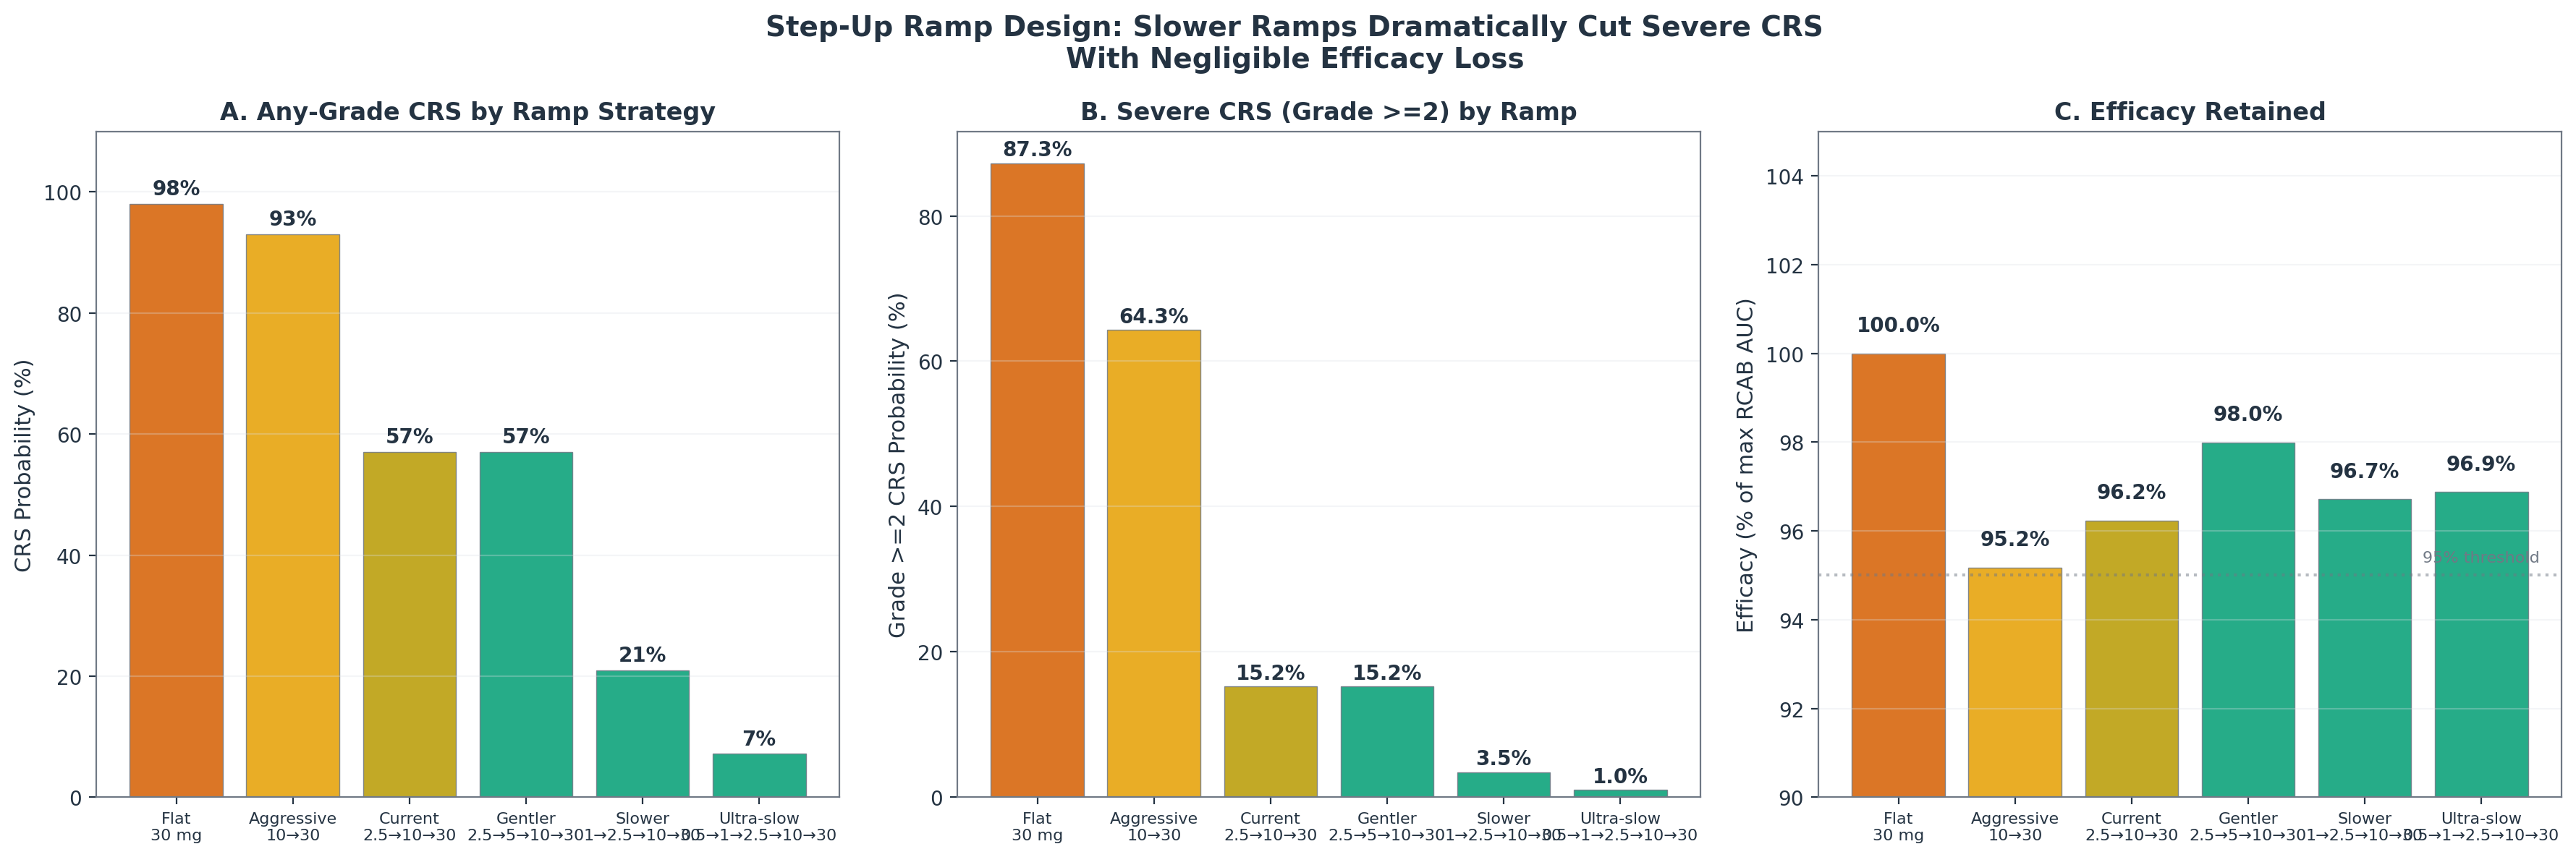
\includegraphics[width=\linewidth,height=.65\textheight,keepaspectratio]{figures/fig3_ramp_comparison.png}
\caption{Step up ramp design affecting severe CRS probability, along with comparison for efficacy retained}
\label{fig:fig3-ramp-comparison}
\end{figure}

Gentler step-up dosing schedules maintain high therapeutic efficacy while significantly reducing the probability of severe CRS. Extremely slow ramping strategies provide additional reductions in CRS risk, though with diminishing returns in efficacy.
\par\medskip

\begin{figure}[H]
\centering
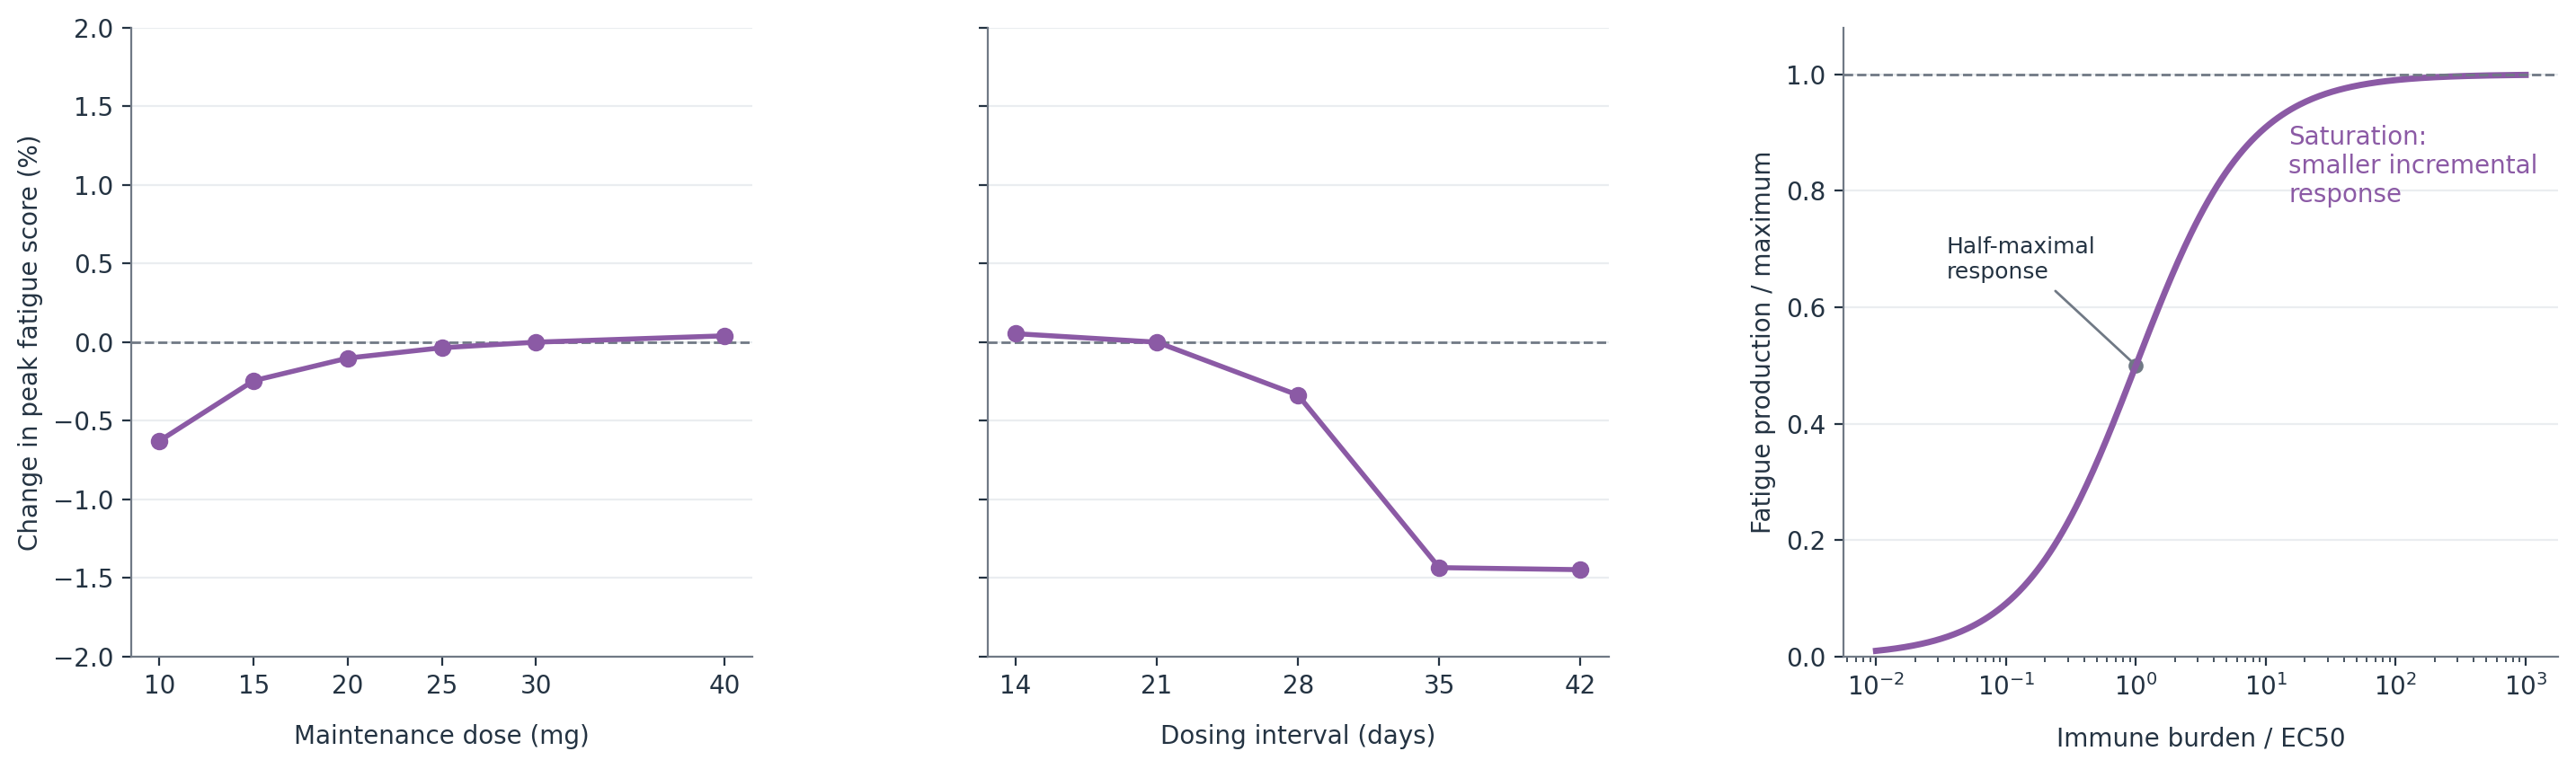
\includegraphics[width=\linewidth,height=.65\textheight,keepaspectratio]{figures/fig4_fatigue_insensitivity.png}
\caption{Predicted fatigue sensitivity to dosing changes. Left: maintenance doses of 10--40 mg. Center: dosing intervals of 14--42 days. Both panels show percentage change in peak fatigue relative to 30 mg every 21 days; absolute peak scores span 1.135--1.143 and 1.126--1.143, respectively. Right: the saturating model response, $b/(b+EC_{50})$, where $b$ is immune burden. Large regimen changes yield small changes in predicted fatigue.}
\label{fig:fig4-fatigue-insensitivity}
\end{figure}

Fatigue remains unchanged despite variations in dose size and dosing interval, indicating a dose-insensitive response.
\par\medskip

\begin{figure}[H]
\centering
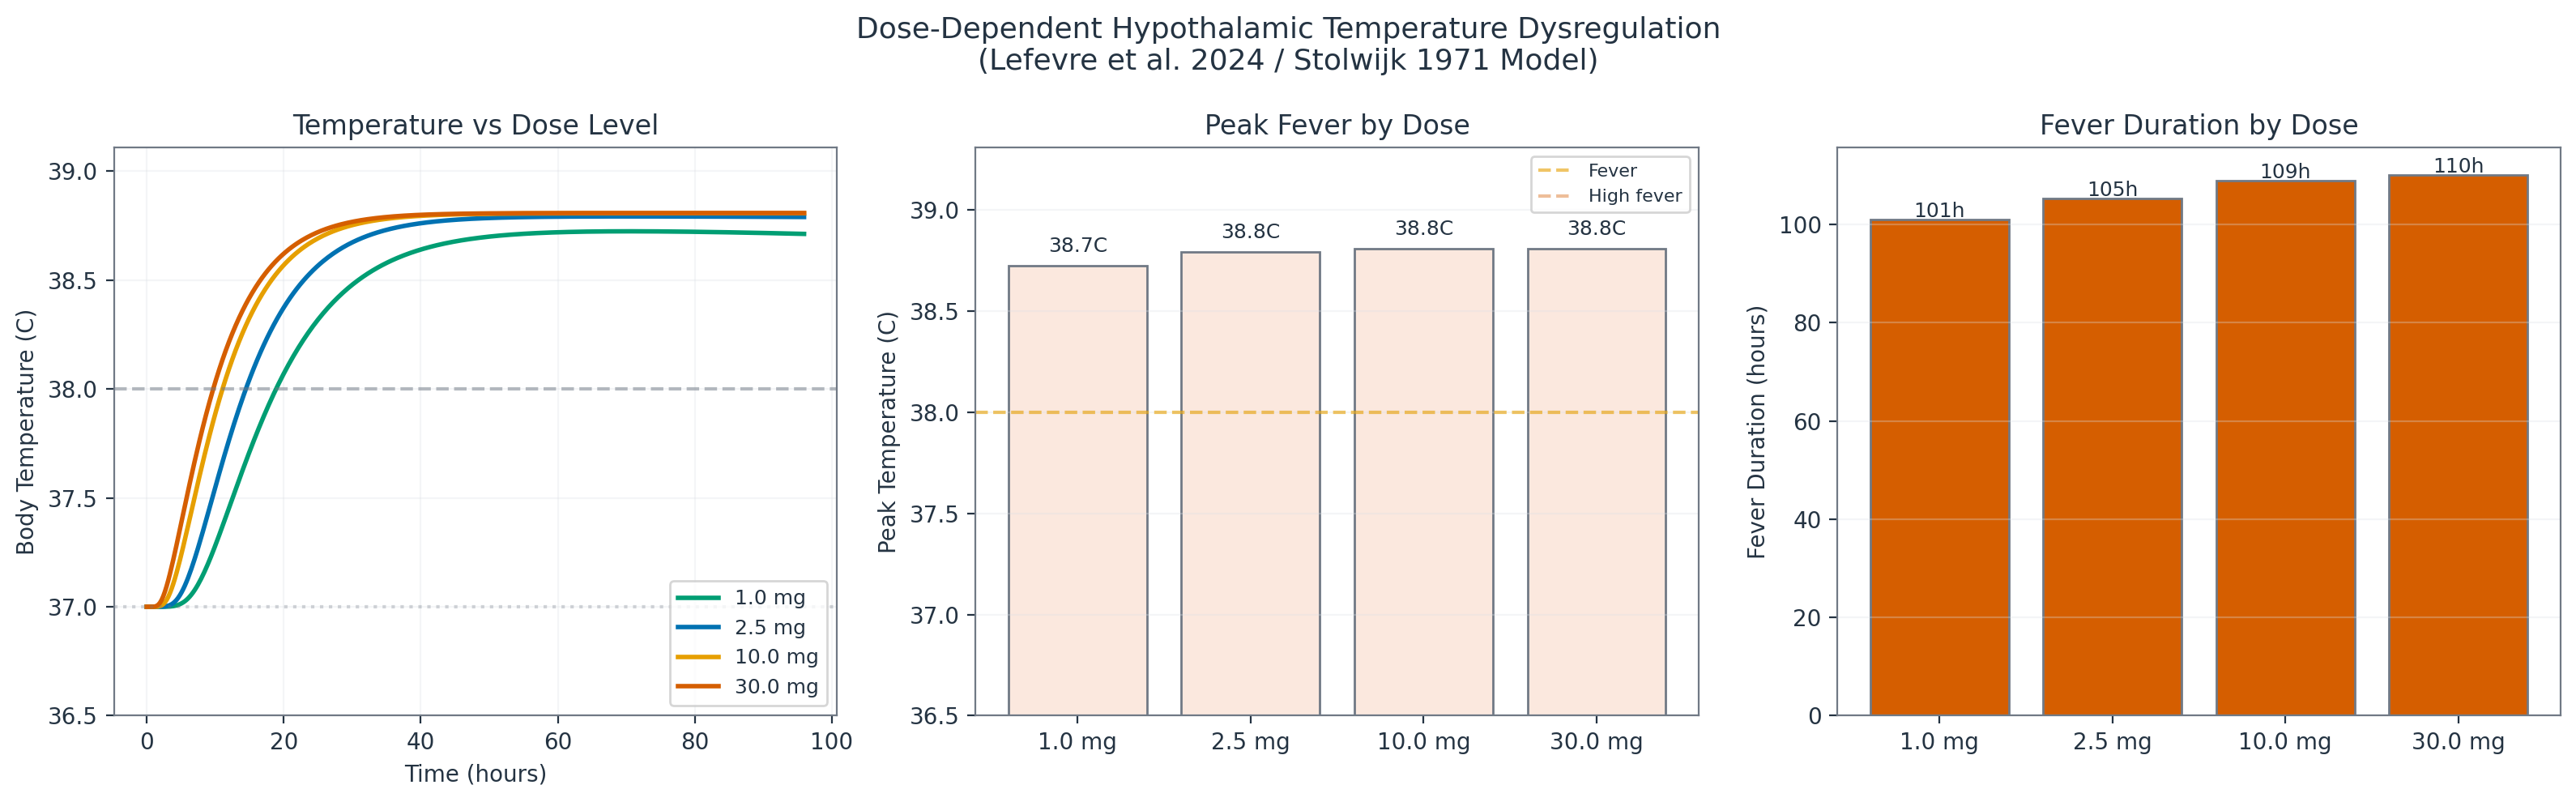
\includegraphics[width=\linewidth,height=.65\textheight,keepaspectratio]{figures/plot10_dose_temperature.png}
\caption{Dose-dependent hypothalamic temperature response in the coupled Lef\`evre--Stolwijk model. From left to right: temperature trajectories, peak fever, and fever duration for 1.0, 2.5, 10.0, and 30.0 mg. Dashed reference lines indicate the fever thresholds.}
\label{fig:plot10-dose-temperature}
\end{figure}

The simulation results demonstrate that the integrated Lefèvre-Stolwijk model successfully captures the dose-dependent kinetics of hypothalamic temperature dysregulation following Glofitamab administration. As shown in the “Temperature vs Dose Level” profiles, the body temperature exhibits a characteristic sigmoidal rise, reaching a plateau that correlates with the escalating dose levels. Notably, even at the lowest simulated dose of 1.0 mg, the model predicts a peak temperature of 38.7°C, crossing the clinical threshold for Grade 1 CRS. As the dose increases to 30.0 mg, the peak fever stabilizes at approximately 38.8°C. This plateau suggests a saturation effect in the cytokine-to-hypothalamic signaling pathway, likely due to the logarithmic nature of the set-point equation, which mimics the physiological saturation of human pyrogenic receptors.
\par\medskip

Furthermore, the model reveals a significant relationship between drug dosage and fever duration, with the recovery period extending from 101 hours at 1.0 mg to 110 hours at 30.0 mg. This prolonged elevation highlights the “thermal inertia” inherent in the Stolwijk passive system; as higher drug concentrations maintain elevated IL-6 levels for longer periods, the hypothalamic set-point remains high, delaying the transition to the cooling phase governed by Newton’s Law of Cooling. These findings underscore the importance of the initial “priming” dose in clinical settings. By predicting the onset and duration of these thermal spikes, this model provides a mechanistic basis for timing prophylactic interventions, such as antipyretics or tocilizumab, particularly in patients identified as high-risk by their baseline tumor burden and LDH levels.
\par\medskip

\section{Discussion}

\subsection{Role of Cytokine Feedback in CRS Dynamics}

Across our simulations, including ternary complex formation, cytokine dose-response curves (IFN-γ, IL-6, IL-2, IL-10), and clinical readouts (fever and fatigue), CRS sensitivity is driven by the balance of positive and negative feedback mechanisms. Early T-cell activation and ternary complex formation trigger IFN-γ–mediated amplification, rapidly escalating pro-inflammatory cytokines and activating macrophages and monocytes, as reflected in peak IL-6 and IFN-γ curves. In contrast, IL-10 functions as a negative feedback regulator, and its timely induction suppresses excessive cytokine signaling, stabilizing fever and limiting fatigue despite dose variations, as shown in the purple fatigue curves and fever dynamics plots. These integrated simulation outputs highlight how feedback timing and strength shape both molecular and physiological responses, providing mechanistic insight into CRS onset and severity.
\par\medskip

This understanding has direct clinical implications for bispecific antibody therapy. When positive feedback dominates, even small increases in ternary complex formation can provoke disproportionately large cytokine responses and severe CRS. Incorporating negative feedback mechanisms, either naturally through IL-10 induction or strategically through interventions like dose titration or step-up regimens, can prevent runaway cytokine responses, reduce peak levels, and keep clinical symptoms in check. Linking cytokine dynamics to symptom curves provides a clear framework for predicting CRS and optimizing treatment to reduce risk while keeping therapy effective.
\par\medskip

\subsection{Model Limitations and Assumptions}

Despite the mechanistic detail incorporated in this framework, several important limitations should be acknowledged. Many parameter values were either assumed or drawn from literature under varying experimental conditions, which may not fully reflect the specific biological context of Glofitamab as a targeted therapeutic drug. Consequently, model outputs should be interpreted primarily as relative trends and mechanistic insights, rather than precise patient-level predictions.
\par\medskip

In addition, the current model does not account for interpatient variability. Biological heterogeneity in factors such as receptor expression, immune cell abundance, and cytokine response has the potential to substantially influence clinical outcomes. The absence of this variability limits the model’s ability to capture the full spectrum of possible observed patient responses. Furthermore, this works represents the immune system through a simplified lens, omitting complex and key regulatory pathways. Thus, this work has a limited ability to fully reproduce the complexity of factors affecting immune activation and dysregulation during antibody therapies.
\par\medskip

Taken together, these limitations highlight that the proposed framework is best interpreted as a mechanistic and hypothesis-generating model, rather than a fully predictive clinical tool. However, these limitations also provide clear directions for future work and improvement. Addressing these constraints through incorporation of patient-specific variability, integration of spatially resolved modeling approaches, and refinement of parameter estimation using clinical datasets will be essential for advancing model fidelity. In particular, improving the representation of immune heterogeneity and toxicity dynamics will be critical for capturing the complexity of clinical outcomes. The present framework serves as a foundational framework for which more physiologically realistic and clinically actionable models of bispecific antibody therapy can be developed.
\par\medskip

\subsection{Future Directions}

Building on the limitations identified in this work, future efforts should focus on extending the current framework into a more physiologically realistic and clinically predictive model. While the present work captures key features of multivalent binding, ternary complex formation, cytokine release, and hypothalamic temperature dysregulation, several important directions remain for further development. In addition, weight loss mechanisms were examined conceptually through literature review, but were not explicitly implemented or tested in the current framework, and thus remain an important direction for future model development, simulation, and validation.
\par\medskip

A primary area for improvement is the incorporation of patient specific variability in receptor expression, baseline cytokine levels, and drug clearance. These factors are very likely to drive significant differences in CRS severity and treatment across individuals. Incorporating such variability, alongside calibration against clinical datasets will also strengthen parameter identifiability and improve confidence in the predictions of the model.
\par\medskip

Another important direction is the refinement of downstream toxicity modeling, particularly for fatigue. Rather than relying on a direct dependence on dose alone, future models should investigate whether fatigue is better explained by cumulative inflammatory burden, prolonged cytokine exposure, or downstream metabolic stress. It could also be useful to include threshold effects, lag dynamics, and recovery compartments since fatigue often appears as a delayed and persistent symptom rather than an immediate acute response.
\par\medskip

Finally, future studies should leverage this expanded framework to evaluate optimized dosing strategies that balance therapeutic efficacy with toxicity mitigation. Such efforts will enable rational design of dosing regimens that minimize CRS risk while preserving anti-tumor efficacy, ultimately supporting the translation of mechanistic modeling approaches into clinically actionable tools.
\par\medskip

\subsection{Further Model Testing and Simulation}

Further testing of the model should focus on systematically exploring how dosing design changes the balance between efficacy and toxicity. Additional simulation should target the downstream toxicity modules, and the hypothalamic temperature model should be challenged under a wider range of cytokine profiles to determine whether the timing and magnitude of simulated fever remain physiologically reasonable across mild, moderate, and severe inflammatory scenarios.
\par\medskip

Likewise, the fatigue model requires further testing because the current results indicate that fatigue did not change by a large amount when dose size or spacing was varied. Simulations for further research should test alternative fatigue structures tied to cumulative cytokine response, duration of fever, repeated T-cell activation, or delayed inflammatory recovery. These results can then be compared to determine which model best reproduces clinically plausible trends.
\par\medskip

Finally, the model could also be further tested with validation oriented simulation studies that compare outputs across the linked submodules. Testing should confirm whether predictions remain internally consistent across short timescale binding dynamics and also longer timescale outcomes. Any additions should conform to the existing findings or provide other mechanistic explanations. In this way, further model testing will improve confidence in the integrated framework and help refine it into a predictive tool for treatment design.
\par\medskip

\section{Appendix}

Tables and citations are available here: \url{https://docs.google.com/document/d/1TBuxTPJg9zp_3K0JgFu_k3pjpyx64Na5BnBF_wPYApE/edit?usp=sharing}
\par\medskip
\end{document}
